\title{\papertitle}

\author{Can Paul Bineytioglu,
		Joe Andr\'{e} Boden,
		Rocco Schulz,\\
		Max V\"{o}kler,
		Robert Wawrzyniak}
		
\publishers{Corporate State University\\Baden-Wuerttemberg - Stuttgart}

\date{\today}

% DOCUMENT

\begin{document}
\pagestyle{scrheadings}

% roman numerals
\renewcommand{\thepage}{\Roman{page}}
% page numbers centered on top:
\chead{\pagemark}
\cfoot{}

%----------------------------------------------------------------------------
% Title Page
%----------------------------------------------------------------------------


\maketitle
% no page numbering on title page
\thispagestyle{empty}

\begin{abstract}
\textbf{\abstractname}: This paper evaluates asynchronous server technologies
using the more recent frameworks Node.js and Vert.x as references. Strengths and
weaknesses of asynchronous programming models are elaborated to identify areas
where these technologies should be chosen over the common programming
frameworks.
A proof of concept based on Node.js and Vert.x is used to evaluate
non-functional attributes such as maintainability and integration into an
existing application landscape.
\end{abstract}
\newpage






%----------------------------------------------------------------------------
% Table of Contents
%----------------------------------------------------------------------------
\tableofcontents
\newpage


%----------------------------------------------------------------------------
% Abbreviations
%----------------------------------------------------------------------------
% List needs to be indexed after each change.
% This is done by executing the following command:
% ~$ makeindex [filename].nlo -s nomencl.ist -o [filename].nls
\printnomenclature
\addcontentsline{toc}{section}{List of Abbreviations}
\newpage


%----------------------------------------------------------------------------
% List Of Tables
%----------------------------------------------------------------------------
\listoftables
\addcontentsline{toc}{section}{\listtablename}
\newpage


%----------------------------------------------------------------------------
% List of Figures
%----------------------------------------------------------------------------
\listoffigures
\addcontentsline{toc}{section}{\listfigurename}
\newpage

%----------------------------------------------------------------------------
% List of Listings
%----------------------------------------------------------------------------
\lstlistoflistings
\addcontentsline{toc}{section}{List of Listings}
\newpage

% Arabic numerals for page numbering
\renewcommand{\thepage}{\arabic{page}}

% Set page number to 1: 
\setcounter{page}{1} 

\renewcommand{\baselinestretch}{1.4}\normalsize

\section{Introduction}

\subsection{Objectives}
Permanent change is a basic concept and global phenomenon in the IT industry. 
Most recent trends include cloud computing, big data, social media and mobile computing.
The tremendous impact of the latter one is  revealed by a Cisco study, which states that in 2011 the mobile data traffic
doubled the fourth year in a row.\footcite[Cf.]{cisco_2012} Those enormous traffic and the
nature of social media applications raised problems in the common synchronous server technologies.
Since 1996 the Microsoft Internet Explorer supports asynchronous content loading. A popular
asynchronous technology is AJAX (asynchronous JavaScript and XML). It got even more attention when
Google ntroduced a wide deployment of standards-compliant, cross browser Ajax with Gmail (2004) 
and Google Maps (2005).\footcite[Cf.]{Swartz_2005} Since then asynchronous technologies
encountered a steep carrier and are on the way to change the way of our programming.
The main goal of this paper is to identify specific use cases for asynchronous server
technologies. Special emphasis is put on applications in the business environment. 
The authors' intention is to build a working prototype in order to present the advantages and
disadvantages of this rising technology.

%Goal of this paper and structure
The two folded approach - explaining the change in web development and an application in an 
business environment - infers two main programming languages, that are ubiquitous in each
community: Java for the enterprise world and JavaScript for the web developers.
This paper elaborates the concepts behind the young frameworks Node.js, that briefly explained enables running JavaScript on a server, and 
Vert.x, a Java implementation of asynchronous technologies, and analyses their 
technical strengths and weaknesses. Furthermore non-functional attributes will be
evaluated based on two sample implementations in Node.js  and Vert.x.

\subsection{Methodology and Structure}
The whole thesis consists of seven chapters. The first two parts explain the author's motivation and introduces the 
basic concepts of asynchronous technologies, whose use cases are explained in chapter three.
Two prototypes of an insurance purchase webpage are implmented in Node.js and Vert.x in chapter 4.
Having set up an exemplary implementation, there are additional concepts explained that are important in modern web development (e.g. AJAX and WebSockets). Before the outlook and the conclusion summarize the paper, non-functional attributes e.g. maintainability and integration are 
investigated.

\subsection{Problem Description}

In traditional web application development data is transmitted synchronously,
i.e. upon a GET/POST request, so that the result can be displayed only after transmission
and processing are finished.

While maintaining simplicity and
predictability this can cause serious latency when uploading large pieces of
data, most commonly complex forms for registration. Naturally rich content such
as images and videos cause even more delays.

As demand around collaborative access and media richness evolved, this became a
serious bottleneck, essentially preventing these types of applications. On the
client-side (browser-side) developers were able to work around the issue of
synchronous transmission using the XmlHttpRequest object which allows to request
resources programmatically (using JavaScript) while
deferring handling of the response to a callback (see Fig. \ref{img_ajax}\footcite{img_ajax}) thus enabling much more responsive software.

\begin{figure}[hbtp]
\centering
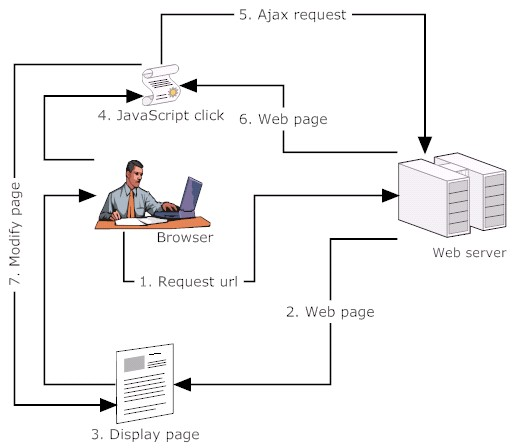
\includegraphics[scale=0.5]{img/ajax-diagram}
\caption[AJAX diagram]{AJAX diagram\label{img_ajax}}
\end{figure}
%\footcitetext{img_ajax}

Although this addressed the issue on the client-side, server-side request were
still handled very much in a synchronous fashion. The Apache web server e.g.
forks a new process for each incoming request\footcite[Cf.][]{apache_2013}.
As popular applications have to cope with unprecedented amounts of concurrent
users in conjunction with massive request counts, this obviously causes
performance issues. Reasons for these issues are that blocking I/O streams also
cause the related thread to idle and consequently block this thread, meaning it
cannot be used for other requests. The next chapter expands upon I/O bound and
CPU bound applications as well as single-/multithreaded technologies, and will
explain further, why asynchronous technologies can help mitigate problems that
especially applications with a lot of I/O streams face.\\

\newpage
\section{Setting the Context}
\label{setting_the_context}

\subsection{Potential Web Development Issues}
\label{potentialissues}
This section is used to briefly outline some theories that are relevant when dealing with synchronous and asynchronous approaches.

\subsubsection{I/O Bound Applications}
\label{issue_io}
I/O bound means that a system requests data faster than the peripheral devices
(e.g. hard disk) can transfer it, causing a process/thread to be put
asleep.\footcite[Cf.][10]{Caldera_2003} The program could be sped up immediately
by faster I/O (e.g. using a Solid State Drive instead of a normal hard disk).

\subsubsection{CPU Bound Applications}
\label{issue_cpu}
CPU bound or compute-bound refers to operations that cause high CPU workload,
like compiling code, spell checking, grammar checking, transcoding audio or
video data.\footcite[Cf.][718]{Richter_2010} They are usually executed in
several threads in order to not block one thread and have all users waiting for
this thread. The program could be sped up immediately by better CPU performance.

\subsubsection{Single-/Multithreading and Event-driven Development}
\label{issue_threads}

% writing multithreaded code is not trivial
In multithreaded applications several threads can run simultaneously within one 
process. Several threads can access shared memory concurrently, which can
cause inconsistent states. This can be avoided by synchronizing threads - e.g.
with locks. This means that programmers need to take into account every possible
execution order to effectively avoid program defects such as data races and 
deadlocks.\footcite[Cf.][10]{Breshears_2009}
This can be time consuming and potentially results in error-prone code.\\

Event-driven programming uses an event loop, which is a single thread that is
running inside the main process.
The loop constantly checks for new events. When an event is detected, the loop
invokes the corresponding callback function. The callback is processed in the
same thread, which means that there is at most one callback running at a time.
The event loop continues when the callback has completed. As a result the
developer does not need to take care of concurrency issues during development.
But the developer's task is to write light event handlers that can be processed
quickly as every callback is an interruption of the event processing in the
event loop. \footcite[Cf.][]{Croucher_2010} Memory or processor intense callbacks
can lead to growing queues of unserved events, which eventually results
in a slow application or service\footcite[Cf.][48]{teixeira_2012}.

\subsection{Concept of Synchronous Processing}
\label{concept_sync}
\FloatBarrier

\begin{figure}[hbtp]
\centering
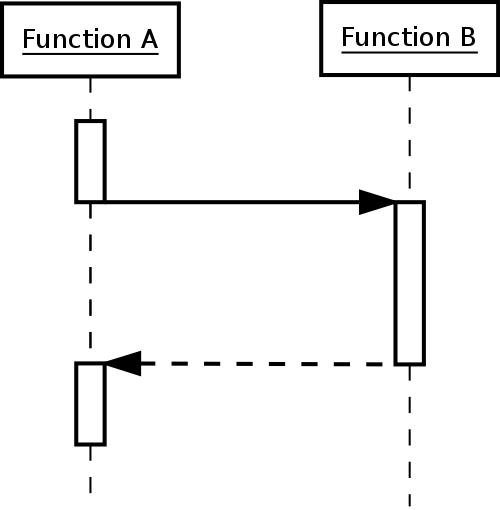
\includegraphics[width=0.4\textwidth]{img/synch_call.png}
\caption{Synchronous, blocking function call}
\label{fig:synch_call}
\end{figure}

In synchronous processing a running thread needs to wait for the completion of
the I/O operation before it can continue.
The thread is in an idle state while it is waiting, which allows another process 
or thread to occupy the CPU in the meanwhile.
\FloatBarrier
\subsection{Concept of Asynchronous Processing}
\label{concept_async}
\FloatBarrier

\begin{figure}[hbtp]
\centering
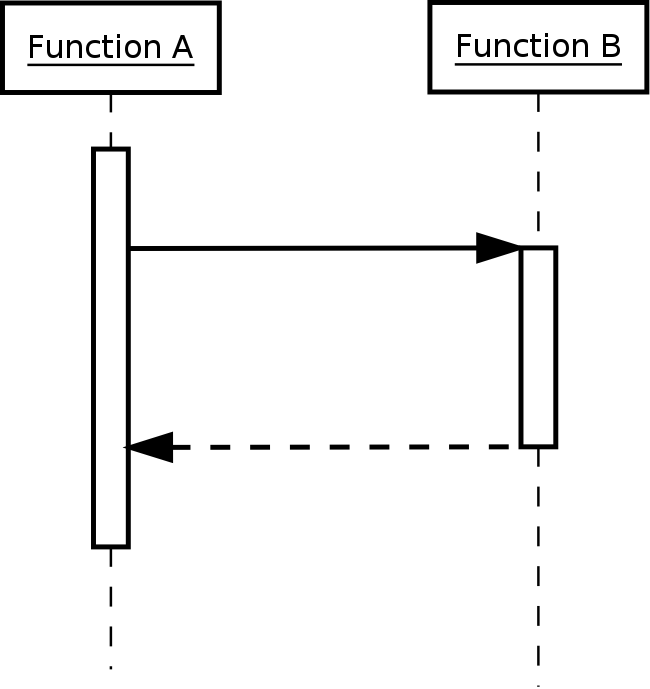
\includegraphics[width=0.4\textwidth]{img/asynch_call.png}
\caption{Asynchronous, non-blocking function call}
\label{fig:asynch_call}
\end{figure}

An asynchronous programming style uses a different concept. The flow of an
application is determined by events, which is why this style is also called
event-driven programming.\footcite[Cf.][16]{teixeira_2012} Asynchronous processing means
that the executing thread is not blocked. There is no
return value - instead an event handler is provided as a second argument.
This function is also referred to as a callback function. It is called as soon
as the read operation has completed and is processed in the same thread, which
means that there is at most one callback running at a time and the developer
does not face concurrency issues.
The developer’s task is to write lightweight event handlers that can be
processed quickly as every callback is an interruption of the event processing
in the event loop.\footcite[Cf.][]{Croucher_2012} Memory or processor intense
callbacks can lead to growing queues of unserved events, which eventually
results in a slow application or service.\footcite[Cf.][48]{teixeira_2012}


\subsection{Technical Comparison of Asynchronous and Synchronous Processing}
\label{comparison_syncasync}

% code goes here...

A typical synchronous call is provided in \autoref{lst:synchronous_call}. The
content of a file is read and displayed afterwards. The program is blocked until the
read operation has finished.

% reading a file and displaying it, pseudo code
\lstinputlisting[language=JavaScript,caption={Pseudocode: Synchronously reading and displaying a file's content},
label=lst:synchronous_call]{lst/synchronous_call.txt}

As opposed to the synchronous call, \autoref{lst:asynchronous_call} demonstrates
how the same example can be realized in an asynchronous fashion using the event-driven
methodology: After the file was read, the callback is triggered in order to
display its content.

% same example as above but with callbacks / events
\lstinputlisting[language=JavaScript,caption={Pseudocode: Asynchronously reading and displaying a file's content},
label=lst:asynchronous_call]{lst/asynchronous_call.txt}


% implication: 
% all code should be as non-blocking and asynchronous as possible
% using blocking APIs inside the asynchronous code can cause blocking of the event loop
% which is evil. This is why Node.js is based on javacript. Other languages already have
% lots of modules with blocking APIs which could confuse dumb developers.


\subsection{Existing Asynchronous Frameworks}
\label{existing_frameworks}
The principle of asynchronous processing has existed on the client-side for a long time and has also evolved
on the server-side. This section will give a brief market overview, which is followed by the
introduction of two upcoming frameworks for server-side asynchronous
development: Node.js and Vert.x.


\subsubsection{Market Overview}
\label{frameworks_overview}
\FloatBarrier
Table \ref{tab:existing_frameworks} shows that there is real competition
from established communities (namely the Ruby and Python ones). An important
aspect in determining the potential success of a new technology is measuring the
interest of software developers in the newcomer. Google-developed Google Trends
visualizes the 'search interest', i.e.\ the amount of queries of a particular
subject and related ones\footcite[Cf.][]{g_trends}.

% \begin{figure}[hbtp]
% \centering
% 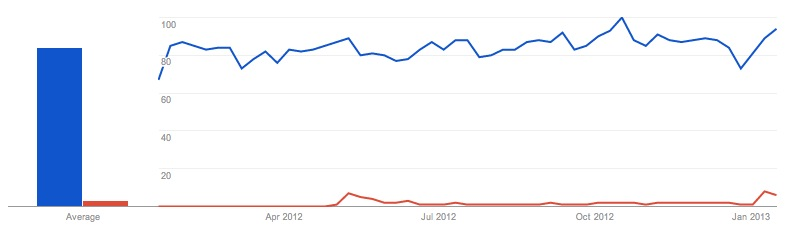
\includegraphics[width=\textwidth]{img/googletrend_nodevertx}
% \caption[Google search volume of Node.js and Vert.x compared]{Google search volume of Node.js and Vert.x compared\}
% \label{img_googletrend_nodevertx}
% \end{figure}
% \footcitetext[Cf.][]{g_trends}

\begin{figure}[hbtp]
\centering
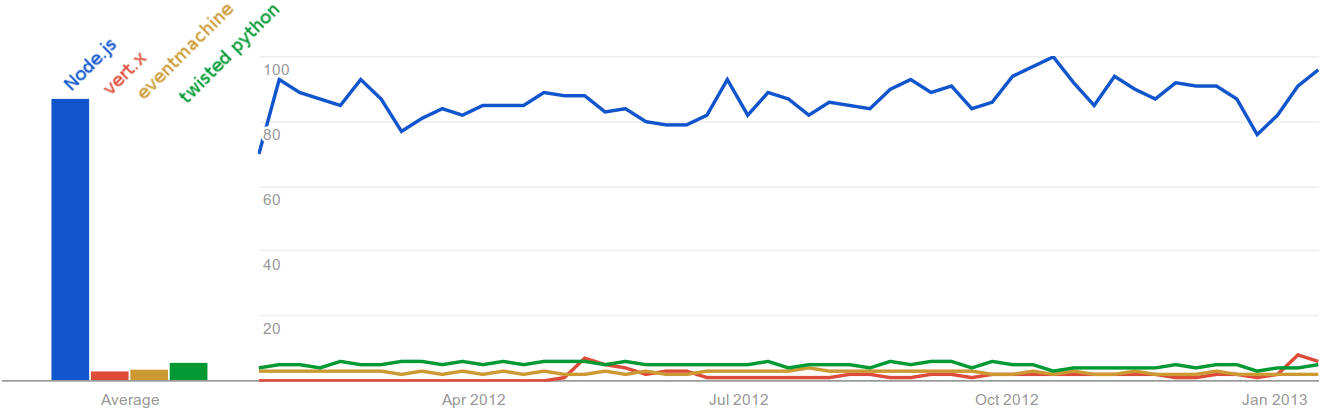
\includegraphics[width=\textwidth]{img/googletrend_all.png}
\caption[Google search volume of Node.js, twisted, eventmachine and Vert.x compared]{Google search volume of Node.js, twisted, eventmachine and Vert.x compared}
\label{img_googletrend_all}
\end{figure}
\footcitetext[Cf.][]{g_trends}

Looking at the graphs in Fig. \ref{img_googletrend_all}, it can be
concluded that interest in Node.js is very high at the moment in absolute terms as well
as in relative terms when comparing it to peers at the same point in there lifecycle.
Interest in Vert.x is comparably low, considering that it's idea is very similar to Node.js.
The gap in interest could be related to many reasons, two of which will be discussed 
briefly thus concluding this section.

Theory (1) would be that by the time Vert.x became complete enough to develop
productively (at least as productive as was possible with Node.js at the same
point), Node.js already established itself as the dominant technology especially if
mindshare is concerned, which is supported by the data from Google.
Theory (2) is based around technical considerations. Because of the dogmatic
nature of asynchronicity in the Node.js framework, every package available on
NPM\nomenclature{NPM}{Node.js Package Manager} is built with asynchronous calling
and non-blocking I/O\nomenclature{I/O}{Input / Output} in mind. Vert.x on the
other hand is in a curious position here. Vert.x itself is architecturally
similar to Node.js but its ecosystem of established Java libraries is not developed
with these principles in mind. This poses the danger of executing
synchronous/blocking code, negating all of Vert.x' advantages. Obviously this
can limit interest from the outset.

Another important metric to assess the potential impact of a framework is the
technical background and the availability of skilled developers. Redmonk
investigated in three consecutive years the popularity of programming languages
by analyzing the usage on GitHub\footnote{See \url{http://github.com}} and
StackOverflow\footnote{See \url{http://stackoverflow.com}}. As of September
2012, JavaScript was ranked first before Java, PHP, Python and
Ruby\footcite[Cf.][]{Redmonk_2012} – all of which have shown a strong
performance over the past three years. This is an affirmative aspect with regard
to the potential target audience of developers of Node.js and Vert.x, which will
be introduced in the next sub-section.


\begin{savenotes} %alloows proper citation marks inside tables
\begin{table}[htbp]
%\begin{longtable}[c]{p{0.2\textwidth} p{0.15\textwidth} p{0.57\textwidth}}
\begin{tabular*}{\textwidth}{p{0.14\textwidth} p{0.15\textwidth} p{0.65\textwidth}}
\toprule
\textbf{Name} & \textbf{Language/s} & \textbf{Description} \\
\midrule 
%\endhead
Twisted			& Python			& ``Twisted is an event-driven networking engine written in 
									  Python and licensed under the open source MIT license"\footcite[Cf.][]{Twisted_2012}.
									  Twisted is a mature framework with a large number of supported networking
									  protocols. Its development is backed by an active
									  community.\footcite[Cf.][12]{fettig_2005}
									  \\
									  
EventMachine 	& Ruby    			& ``EventMachine is a library for Ruby, C++, and Java
									  programs. It provides event-driven I/O using the Reactor 
									  pattern."\footcite[]{eventmachine_2012}\\

Node.js			& JavaScript		& Node.js is based on Chrome's JavaScript runtime \textit{V8}.
									  The platform is fully event-driven and offers core
									  functionalities for network programming. Its functionality
									  can be extended with a large number of modules using an
									  integrated package management system.
									  Node.js started development in 2009 and the community
									  is growing since that.\footcite[Cf.][]{Mashtable_2011}\\
									  
Vert.x			& JavaScript, Java, Python, Groovy, Ruby, Coffeescript		
									& A JVM based platform for network applications which is
									  inspired by Node.js. Vert.x comes with its own event
									  bus system that allows distributing applications
									  among multiple network nodes. Support for the languages
									  Scala and Clojure is scheduled for future releases.\footcite[Cf.][]{vertx_2012}\\
\bottomrule 
\end{tabular*}
  \caption{Existing asynchronous programming frameworks}
  \label{tab:existing_frameworks}
%\end{longtable}
\end{table}
\end{savenotes}

Table\ref{tab:existing_frameworks} only considers four major frameworks. Other libraries/frameworks include, but are not limited to:

\begin{itemize}
  \item Perl's AnyEvent\footnote{\url{http://software.schmorp.de/pkg/AnyEvent.html}}
  \item Ruby's Rev\footnote{\url{http://rev.rubyforge.org/rdoc/}} and Cramp\footnote{\url{http://cramp.in/}} which is built on EventMachine\footnote{\url{http://rubyeventmachine.com/}}
  \item Python's tornado\footnote{\url{http://www.tornadoweb.org/}}, asyncore module\footnote{\url{http://effbot.org/librarybook/asyncore.htm}} and sitting on that Medusa\footnote{\url{http://packages.debian.org/sid/python-medusa}}
  \item Python's gevent\footnote{\url{http://www.gevent.org/}} library
  \item .NET's Rx\footnote{\url{http://msdn.microsoft.com/en-us/data/gg577609}} library
  \item JVM's NIO\footnote{\url{http://docs.oracle.com/javase/1.5.0/docs/guide/nio/}}
  \item Linux' epoll\footnote{\url{http://linux.die.net/man/4/epoll}}, C's libev\footnote{\url{http://software.schmorp.de/pkg/libev.html}} and libeio\footnote{\url{http://software.schmorp.de/pkg/libeio.html}}
  \item Erlang\footnote{\url{http://www.erlang.org/}}
\end{itemize}

\FloatBarrier

\subsubsection{Node.js}
\label{Node.js}

Node.js is a framework based on Google's V8 JavaScript Engine, libUV as platform
layer\footnote{See \url{https://github.com/joyent/libuv}}, and a core library
written in JavaScript.
Node.js brings JavaScript to the server-side and therefore makes it possible to
write a web application on both, the server-side and the client-side in one
language – JavaScript.

Compared to other technologies that try to apply the fundamentals of
asynchronous programming, Node.js' libraries are programmed completely
asynchronous. Its architecture consists of modules to simplify the creation of
complex applications. Modules are encapsulated pieces of code like libraries in
C or units in Pascal. Every module contains of set of functionalities that share
one common purpose. The visibility of functions and variables is limited to the
module they belong to. Using a module requires to call the function \texttt{require()}
and its allocation to a variable.
Every function in Node.js is asynchronous, which means that the current thread
continues running and does not wait for completion (see Fig.
\ref{fig:asynch_call}). Exemplarily, reading a file works in a way that when the
read operation has finished, a callback function is executed to continue working
with the file's content.

Node.js is single-threaded, which is why only one thing can happen at the same
time. Node.js's asynchronous programming style is implemented through events
that determine the flow of execution. The events are processed within an event
loop (see section \ref{issue_threads}). Consequently, the code execution is
thread-safe and there is no issue regarding concurrency that affects the shared
memory state.\footcite[Cf.][p.16]{teixeira_2012}

\begin{figure}[hbtp]
\centering
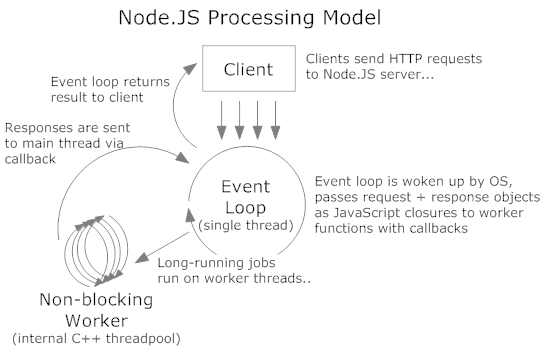
\includegraphics[width=\textwidth]{img/processing_model.png}
\caption[Processing Node.js]{Processing Node.js\footnotemark}
\label{fig:processing_model}
\end{figure}
\footcitetext{aaronstannard_2011}

Node.js's large performance benefits are caused by the use of Google's new JavaScript engine V8, which naturally ships with the web browser Chrome and is used for Node.js too. Due to the fact that V8 compiles JavaScript into
real machine code before executing it, Node.js has an advantage over 
traditional techniques such as executing bytecode or interpreting it.\footnote{See \url{https://developers.google.com/v8/intro}}
\\
Node.js by default provides core modules that are packed in its binary, to help
access files on the file system, create HTTP and TCP/UDP servers, and to perform
other useful functions.\footnote{See \url{http://nodejs.org/api/modules.html\#modules_core_modules}}
The latest version of the Node.js environment can be installed from a GitHub repository.\footnote{See \url{http://nodejs.org/dist/latest/}}
Even though the core modules are sophisticated enough to write complex applications, Node.js is not complex itself.
The node package manager, however, provides 21,104 packaged modules as of
January 18, 2013\footcite[Cf.][]{node_packages}, which enable the developer to
leverage a variety of pre-defined complex functionalities.
Since Node.js version 0.6.3 the package manager npm is deployed and installed
automatically within the environment.\footcite[Cf.]{blog_nodejs_2011} Npm is run on the command
line and manages dependencies for applications.\\
Node.js received standing ovations from the web developer community, which lead
to spectacular participation in the project. Primarily, Node.js is supported by
a San Francisco based company named Joyent, which offers cloud services such as
Infrastructure as a Service and Platform as a Service to large companies,
focussing on open-source projects such as Ruby on Rails and
Node.js.\footcite[Cf.][]{jaxenter_2010}\\
Node.js's documentation and manual are extensive and cover all functionalities
of the non-extended edition.
Node.js is licensed under the MIT License\footnote{See
\url{http://opensource.org/licenses/MIT }}, meaning that it permits reuse within
proprietary software provided all copies of the licensed software include a copy
of the MIT License terms.\\



\subsubsection{Vert.x}
\label{Vert.x}

Vert.x is a programming framework that runs on the Java Virtual Machine (JVM).
It is hence possible to scale over
available cores without manually forking multiple processes.\\
The application API is exposed in multiple programming lanugages (see table
\ref{tab:existing_frameworks}).
% Implication: use case, code reuse from different legacy systems written in
% different languages

In Vert.x the smallest available deployment unit is a verticle, which runs
inside an instance. Each instance runs single-threaded.
Multiple verticles can be run inside one instance as depicted in Fig.
\ref{fig:vertx_constructs}.

\begin{figure}[h]
	\centering
	\setlength\fboxsep{2pt}
	\fbox{
	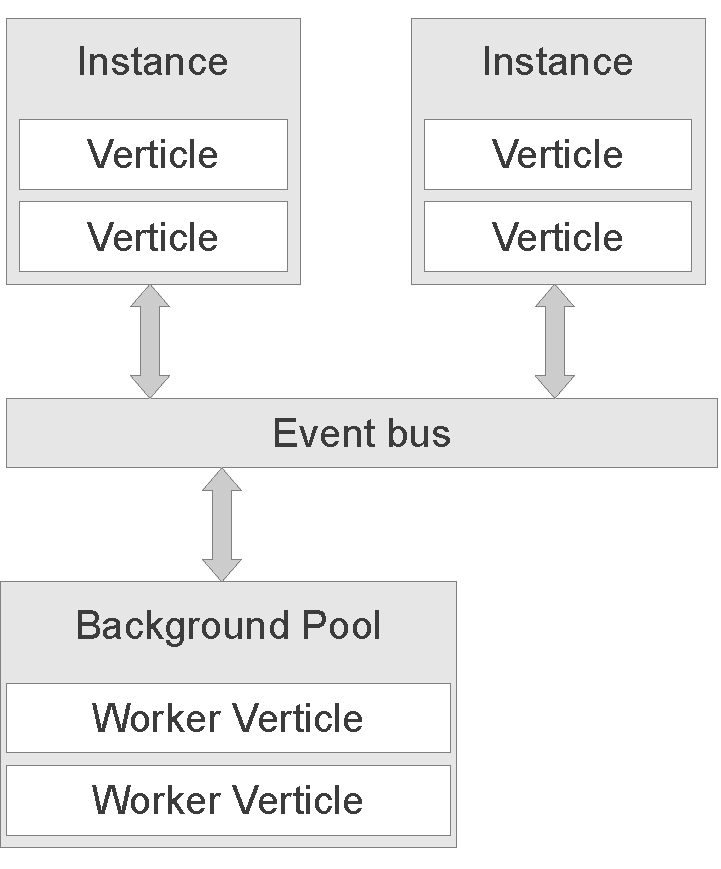
\includegraphics[width=0.4\textwidth]{img/vertx_constructs.pdf}
	}
	\caption{Abstracted deployment units of Vert.x}
	\label{fig:vertx_constructs}
\end{figure}

When multiple instances are run on one machine, Vert.x automatically distributes incoming
requests among all running instances in a round-robin fashion, so that each
Vert.x verticle instance remains single-threaded. Technically seen, there is
more than one event loop, but Vert.x employs a mechanism that ensures that all events
that are related (e.g. because they triggered each other) are run in the same context, i.e. the same thread.
This allows real concurrency while providing the benefits of single-threaded programming style.

Vert.x also includes a distributed event bus, which enables verticles to
communicate with each other, either within the same instance or across different
instances. The event bus allows direct communication with in-browser JavaScript as well.
Vert.x uses the SockJS library for this purpose which is a wrapper around normal websockets with a
fallback to alternative technologies, such as long-polling\footcite[Cf.][]{sockjs_2013}.
This is shown schematically in Fig. \ref{fig:server_bridge}.

Vert.x allows to run I/O heavy tasks in separate worker threads that reside in a
so-called background pool as these tasks would otherwise block the event loop as
described in section \ref{issue_threads}.

\begin{figure}[htb]
\centering
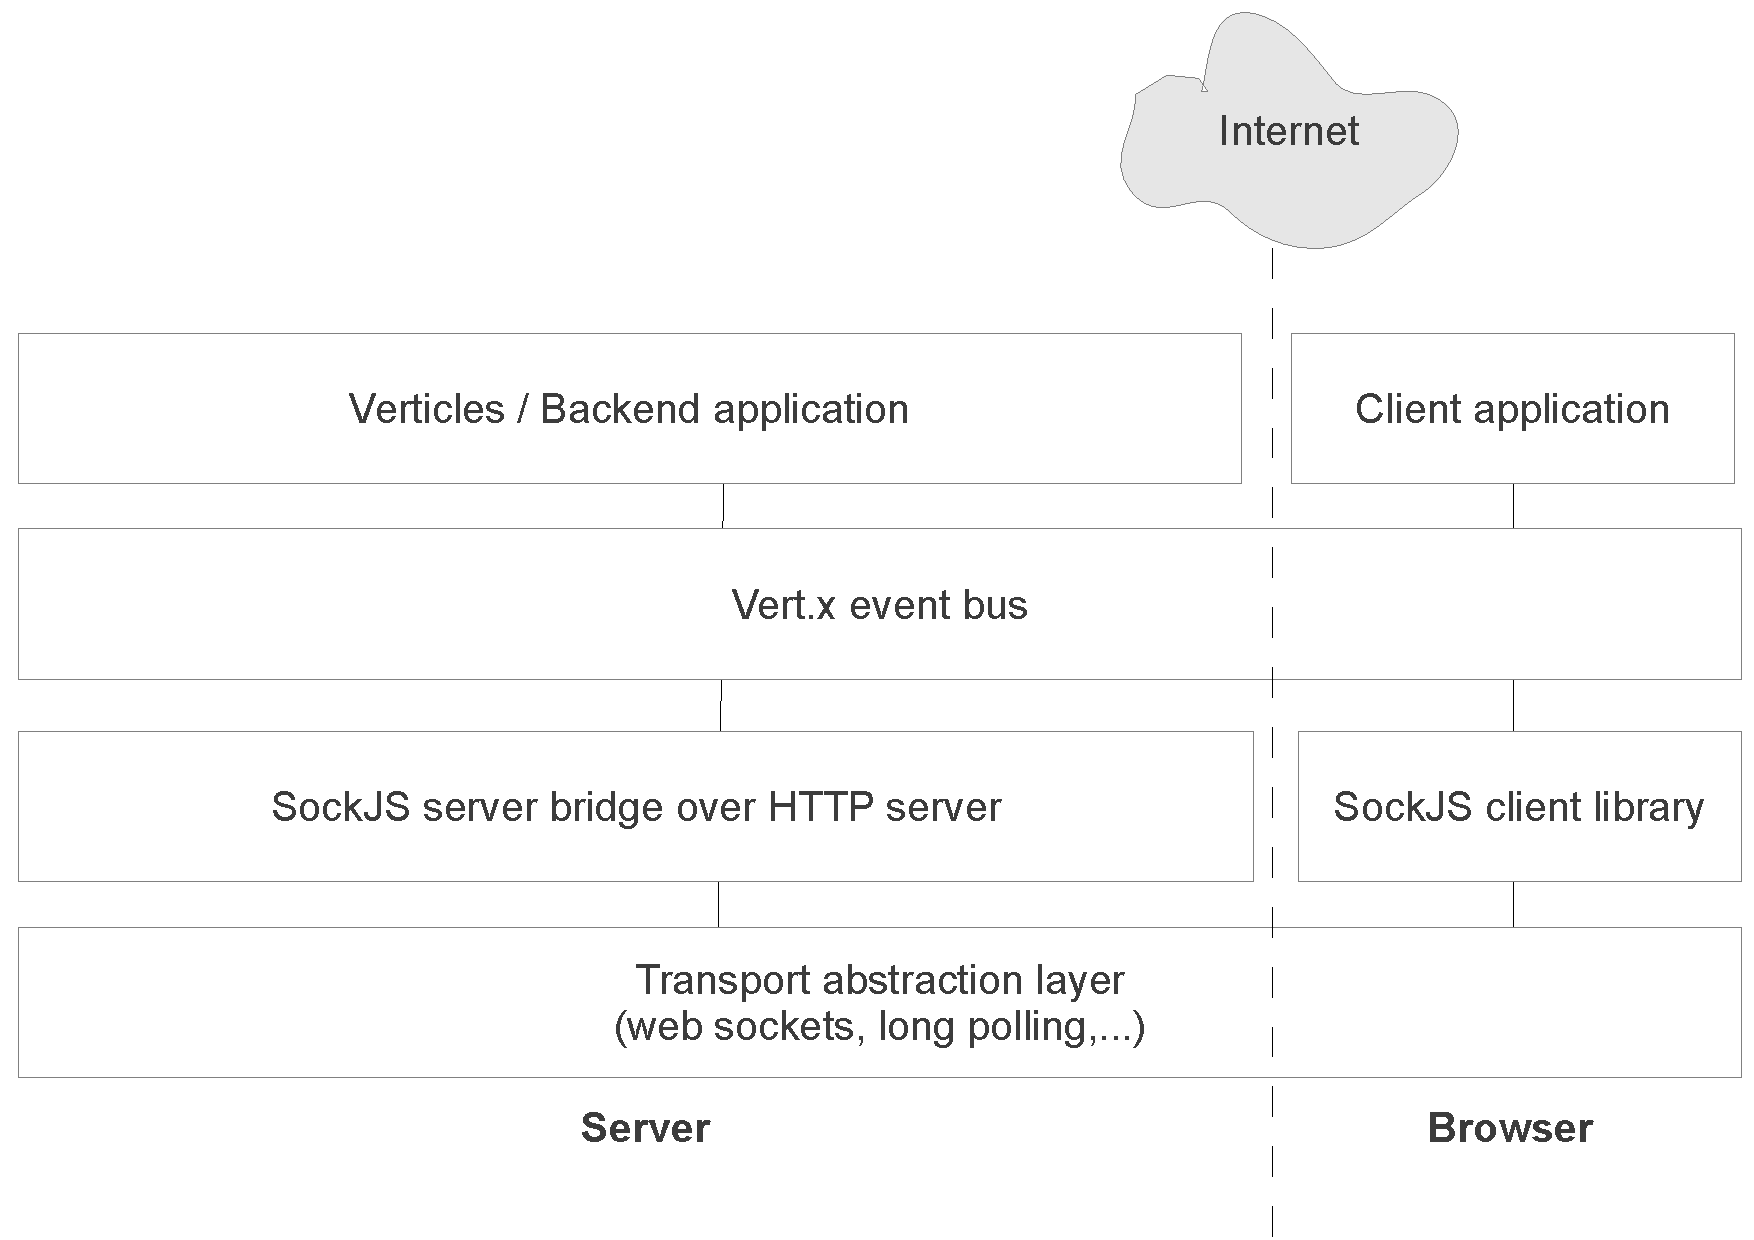
\includegraphics[width=0.7\textwidth]{img/vertx_server_bridge.pdf}
\caption[Vert.x server bridge]{Vert.x server bridge - schematic view}
\label{fig:server_bridge}
\end{figure}
%
The core functionality of Vert.x covers basic networking tasks and protocols,
web servers, network clients, access to the file system, shared maps and the event bus.
The core libraries of Vert.x can be embedded in any JVM program for reuse in
larger projects.\\
As opposed to Node.js, the core functionality and API can be considered quite
stable as changes need to be done in all supported languages.\footcite[Cf.][]{vertx_2012}\\ % The core can be extended with
The core can be extended with additional features that are provided by optional
modules which can be obtained over a public git-based module
repository.\footcite[Cf.][]{vertx_mod_2012}.
The repository currently contains 16 distinct modules in different
versions.\footcite[Cf.][]{Vertx_repository_2012} Compared to Node.js this
number is very low and reflects the relatively low interest in the project
in comparison to Node.js (see Fig. \ref{img_googletrend_all}).
However one should bear in mind that many libraries available for the languages supported
by Vert.x can be used within this framework as well.

An extensive online documentation is available for all supported languages.
Additionally, code examples for most features are available for all supported languages in
a public repository\footcite[Cf.][]{Fox_2013}.\\
Vert.x is open source and licensed under the Apache Software License
2.0\footnote{See \url{http://www.apache.org/licenses/LICENSE-2.0.html}}, so that
commecial redistribution in closed source projects should not be an issue.
At present the project is owned by VMware, but it is likely that it will be transferred to
an Open Source foundation (see section \ref{vertx_maintainability}).


\newpage
\section{Areas of Application}
\label{areas_of_application}

\subsection{Use Cases}
\label{use_cases}
The non-blocking nature of asynchronous calls is important in all types of
applications that need to handle a large number of requests. Its event-driven model
also makes it a good choice for most types of real time processing.\\
A fairly obvious fit is given for I/O bound applications, as the single-threaded asynchronous processing
does not wait for I/O streams to finish, but instead uses callbacks to come back to the processing part
as soon as the I/O has finished.
The single-threaded nature of event loops allows to make efficient use of the
thread as long as callback functions don't take up too much time. This makes asynchronous
server applications a good fit for most types of networked applications that
either tend to keep many inactive connections or need to handle many concurrent 
short-lived connections.

A few possible use cases are described in the list below. Furthermore case studies of real
implementations are provided in appendices \ref{app:case_linkedin}, \ref{app:case_aircode},
\ref{app:etherpad} and \ref{app:case_clock}.


\begin{description}
\item[Web traffic monitoring] By getting notified of every single request that
arrives on an online service, an asynchronous application could keep track of the
current number of requests and the distribution of requests among all
available resources. These simple statistics could then be pushed to a Web interface
frequently to allow real time monitoring of a service in the browser.\\
\textbf{Realization:} All services that should be monitored could implement a
middleware that intercepts each request and fires a call to the asynchronous
server. However that would add a lot of overhead for the services that should
be monitored. Alternatively all clients that access these services could be forced to send a
second request to the asynchronous server.\\
The asynchronous server instance could then handle each request by adding
relevant information to an in-memory database. In the case of HTTP requests
these information could simply be taken from the various HTTP header fields.
\footcite[Cf.][]{http_rfc}\\
A second server instance could be set up to handle the online dashboard.
In order to allow instantly updating the dashboard all clients should be
connected to this instance via a WebSocket (described in section \ref{websockets}). Depending on the amount of visitors
this could result in a large number of open connections. However due to the
event loop based processing the server instance will always just use one
thread for all connections as opposed to a classical web server, which would
keep one thread for each connection. Thus the servers footprint is much
smaller.\\
\textbf{Known implementation:} Hummingbird is a real time web traffic
visualization tool that uses Node.js for all processing. When loading a
website the browser sends a request for each file that is referenced in the
HTML file. Hence each page that should be tracked by Hummingbird integrates a
reference to a tracking pixel, which is served by the Hummingbird application.
\footcite[Cf.][]{hummingbird}. The dashboard is updated 20 times a second
over a WebSocket connection.

\item[Streaming] Applications that involve a lot of streaming of data, such
as file uploading or video broadcasting, represent another appropriate use
case for asynchronous technologies. Especially Node.js uses an abstraction
called streams. Such a stream represents a flow of data and can appear as a
readable stream or writable stream.\footcite[Cf.][75]{teixeira_2012} Why
Node.js is beneficial in terms of streaming data becomes clear when
considering the slow client problem and the way Node.js and its streams
address it.\\
\textbf{Realization:} The slow client problem refers to the scenario where a
process reads data, processes it and sends it to another consumer.\footcite[Cf.][80]{teixeira_2012}
If the producer (readable stream) sends data faster than the consumer (writable stream)
can process it, the data has to be buffered. For instance, consider uploading
a local file: The readable stream is relatively fast as the file is stored locally.
Assuming the network connection to the client is slow, the writable stream will consequently
be slow as well. As a result, the data has to be buffered. Because data will be buffered in
memory for each write command, this will result in memory problems after a certain amount of
requests.\footcite[Cf.][81]{teixeira_2012} This problem can be avoided by pausing the producer
until the consumer catches up. At this point, Node.js comes into play. Readable streams
in Node.js can be paused and resumed, which addresses exactly the described
problem.\footcite[Cf.][81]{teixeira_2012} Listing \ref{lst:streaming} illustrates
how this is realized.\footcite[Cf.][81]{teixeira_2012}

\begin{lstlisting}[language=javascript,caption={Controlling streams in Node.js},label=lst:streaming]
require('http').createServer(function(req, res) {
var rs = fs.createReadStream('/path/to/big/file');

rs.on('data', function(data) {
if (!res.write(data)) {
rs.pause();
}
});

res.on('drain', function() {
rs.resume();
});

rs.on('end', function() {
res.end();
});
}).listen(8080);
\end{lstlisting}


The data flow control process can be automated by using the
\texttt{stream.pipe()} method.
\textbf{Known implementation:}
Transloadit\footnote{\url{http://transloadid.com}} is a company offering a
solution for file-uploading and encoding. They have implemented their service
in Node.js and take advantage of the functionality of Node.js’s streams. Also
Yahoo uses Node.js for file uploads.\footcite[Cf.][]{Odell_2012}


\item[Lightweight network servers] Asynchronous technologies are a good fit
for HTTP servers and are efficient when it comes to handling many concurrent
connections in a single process. A web server application should handle
the cookie header parsing, maintainance of sessions, serving static files,
parsing the request body etc.\footcite[Cf.][197 et seq,]{teixeira_2012} Most of these
tasks are very simple and don't require much computations.
The Proof of Concept also shows that other
protocols, like WebSockets, can take a particular advantage from asynchronous
technologies. In general any network server that only needs to handle a small set of
tasks could be written easily using one of the mentioned frameworks.\\
\textbf{Realization:} The realization can be seen exemplarily in listings
\ref{lst:includenodemodules} et sqq., as this is part of the Proof of Concept.
\textbf{Known implementation:} 
\textit{Connect}\footcite[Cf.][]{Odell_2012} is a well-known Node.js-based middleware that provides
webserver functionality and is considered an industry
standard.\footcite[Cf.][145]{Roden_2012} For Vert.x, there is a
webserver project called \textit{mod-web-server}\footcite[Cf.][]{vertxmodwebserver_2013}, which
efficiently serves files and can also be configured as en event bus bridge to
client-side JavaScript.\\


\item[Proxies] There are two indicators that militate in favor of an asynchronous server:
Proxies usually handle a large number of requests and secondly they mainly do I/O related work
but no big computations. A common task might be to filter a set of URLs, which can be
easily done with an array in Java and JavaScript.\\
\textbf{Realization:} The requests are caught intercepted by the proxy server, which then
requests the actual website and passesit back to the requesting
client. Other requests can be handled while the resources are being loaded.
There are examples of Node.js showing a proxy written on 20 lines of code\footcite[Cf.][]{krumins_nodeproxy}.
These implementations could be extended to provide more sophisticated features.
\textbf{Known implementation:} There is a Vert.x implementation called
\textit{vertx-proxy}\footcite[Cf.][]{vertxproxy} as well as a Node.js proxy called
\textit{node-http-proxy}\footcite[Cf.][]{nodeproxy}, both of which support HTTPS.\\

\item[Push-notification and messaging systems] Asynchronous technologies are
suitable for web applications and networking tools that have to handle many
concurrent connections as they are event-driven.\footcite[Cf.][17]{teixeira_2012} Such applications process a
high number of requests fast, which in most cases means in real time. At the
same time, the tasks are not CPU-intensive and do not block the event loop. \\
\textbf{Realization:} Such web applications or services can include chat
platforms, sport bets, e-mailing and instant messaging
applications.\footcite[Cf.][]{GeisendoerferF_2011} As opposed to synchronous
processing, the event-loop keeps working while notifications are delivered to
clients and potential callbacks are processed as soon as messages were received.
As everything occurs in a single thread, an overhead of switching threads and
concurrency issues can be avoided.\\
\textbf{Known implementation:} \textit{AIRCODE} has implemented such a real time
notification application entirely in Node.js (see Appendix \ref{app:case_aircode}). Moreover,
financial applications that need to show immediate reaction to stock
changes may take advantage of asynchronous processing to implement real time notification systems.

\end{description}

\nomenclature{URL}{Uniform Resource Locator}


\subsection{Inappropriate Use Cases}
\label{dont_use_cases}

As with all technologies one has to carefully evaluate whether or not it suits the
requirements of a project. Besides those use cases listed in the previous
section there are also a few usage scenarios where one should not use
asynchronous frameworks like Node.js or Vert.x. In general, the choice
always depends on the very specific needs for every single use case.
Critics argue that asynchronous frameworks are not necessarily the best choice
only because they represent a new stream.\footcite[Cf.][]{semerau_2011}\textsuperscript{,}\footcite[Cf.][]{arranz_2011}\textsuperscript{,}\footcite[Cf.][]{behren_2003}

Since one key feature of asynchronous technologies is non-blocking I/O, use
cases that hardly encompass interaction with external resources do not set a
precedent and might even be penalized. This penelization would be caused by the
fact that the strength of non-blocking I/O could not be leveraged on the one
hand and on the other hand one thread would be busy through computations and
cause long response times.\footcite[Cf.][14]{Roden_2012}

Expanding upon the non-blocking I/O strenghts, it becomes obvious that
asynchronous frameworks are not I/O bound. Consequently, they are not
designed to deal with CPU bound use cases.\footcite[Cf.][15]{Nguyen_2012}

\begin{description}
  \item[Datawarehousing with analytics] Doing analytical and complex computations
  	on large data sets at runtime usually requires a lot of computing power.
  	It can be expected that each request will require quite some time to be processed.
  	This computation time cannot be shortened much when run on a single thread but 
  	could potentially be sped up significantly when run on multiple cores in parallel. 
  \item[CRUD / HTML applications] \nomenclature{CRUD}{Create Read Update Delete}
	This refers to classical websites that basically only serve as an interface for
	an object relational model.
	At present Node.js and Vert.x do not provide additional benefits to scalability
	for these types of web applications.\footcite[Cf.][15]{Roden_2012} Unless the page has to deal with a large number of
	concurrent requests it should be considered to use more powerfull frameworks
	like \textit{Ruby On Rails}, \textit{Grails} or \textit{Django}. These are currently better suited for quickly
	developing such an application. Providing a site that is suited for 
	millions of requests per day does not automatically increase the number of users.
  \item[XML-based environments] This applies for Node.js in particular. Node.js makes strong use of JSON as a data format and
  does not support XML. Node.js should hence not be used in an environment that communicates in data formats like XML.
\end{description}

This leads to the simple conclusion that migrating from legacy applications to asynchronous
server applications can neither be justified by the benefits that asynchronous technologies
can offer, nor by the hype around these frameworks alone. The true indicator should be whether
or not it is the best suited technology for the application area in the given enerprise context.
    


\newpage
\section{Exemplary Implementations}
\label{exemplary_implementations}

A simple web form application has been implemented in both Node.js and Vert.x to
further analyze non-functional requirements and collect practical experience
with these frameworks. These implementations are thoroughly described in the following sub-sections.

\subsection{Software Description}
\label{software_description}
\FloatBarrier
The exemplary implementation consists of a web service that can be used to calculate
the expected fee for an insurance. The idea behind this application is that
two clients can collaborate during the form entry process before submitting
all values for the fee calculation to the server.
However this application should only serve as a demonstration of the used asynchronous 
frameworks and is hence very simplified.\\
Functionalities that are included are usual POST requests as well as real time communication
via a WebSocket (described in section \ref{software_design}).

\begin{figure}[h]
	\centering
	\setlength\fboxsep{2pt}
	\fbox{
	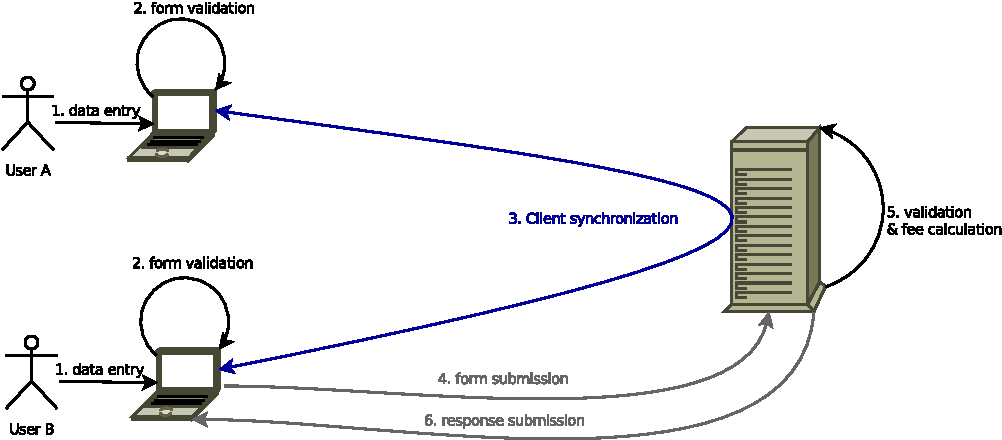
\includegraphics[width=0.9\textwidth]{img/poc_workflow2.pdf}
	}
	\caption{Usage workflow of the exemplary application}
	\label{fig:application_workflow}
\end{figure}


The basic usage workflow is shown in Fig. \ref{fig:application_workflow}.
Upon page load both users can assign a form key. All users with the same key
will be collaborating with each other and receive all input changes from the
other users - this is comparable to a simple chat.
the form consists of two parts - the first part being a section for personal
details and the second part for parameters that will be used to determine the
fee for the insurance.\\
The users then fill in all necessary form fields (step 1 in Fig.
\ref{fig:application_workflow}) and instantly get feedback on the vailidy of the
entered values (step 2 in Fig. \ref{fig:application_workflow}).
The evaluation is done locally on the clients' machines.
While typing the data into the form fields, those inputs are instantly sent to
the server using WebSockets.
The server will distribute these inputs to all clients that have opened the same
form, which is identified via the key that was set initially (step 3 in Fig.
\ref{fig:application_workflow}).\\
Once all fields that are required for the fee calculation are filled correctly
the client automatically submits the values via AJAX to the server over a secure
HTTPS connection (step 4 in Fig. \ref{fig:application_workflow}). On the server
these values are then validated again to avoid processing of manipulated requests
(step 5 in Fig. \ref{fig:application_workflow}). The result of the fee calculation
is then returned to the client, which closes the HTTP connection (step 6 in Fig. \ref{fig:application_workflow}).\\
This AJAX call is triggered when the three fields of the second part (being
\textit{career}, \textit{amount insured} and \textit{ownership stake}) are
valid.\\
Using two different technologies (WebSockets and AJAX) for this workflow is
certainly not the best approach from a design point of view but is conceptually
valuable to show serveral ways of communication.

\nomenclature{HTTPS}{Hyper Text Transfer Protocol Secure}
\nomenclature{HTTP}{Hyper Text Transfer Protocol}
\nomenclature{AJAX}{Asynchronous JavaScript and XML}





\FloatBarrier
\subsection{Software Design}
\label{software_design}

\nomenclature{HTML}{Hyper Text Markup Language}

This simple usage scenario leads to a few requirements and
design decisions.
The user interface has to consist of HTML, CSS and JavaScript files as it 
will be displayed in a web browser. In general these files are not initially
available on the clients machine and need to be delivered via HTTP/HTTPS by the
server. These file requests are usually done via GET.\\

\begin{figure}[h]
	\centering
	\setlength\fboxsep{2pt}
	\fbox{
	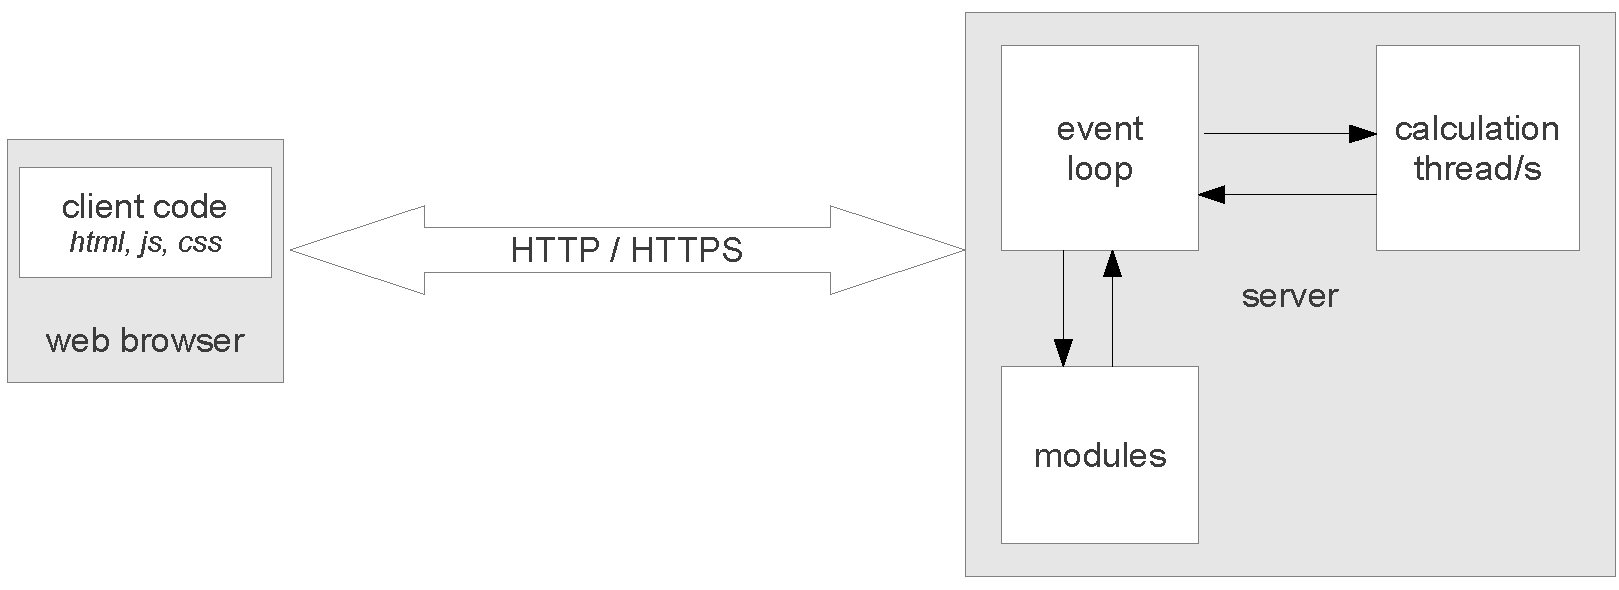
\includegraphics[width=0.8\textwidth]{img/high_level_architecture.pdf}
	}
	\caption{High level architecture of the application}
	\label{fig:high_level_architecture}
\end{figure}

In addition to the static files, the server will also need to process
requests that are sent via POST in order to receive the form data for the
fee calculation.\\
The body size of these requests is fairly small as the submitted values consist
of plain text only. Therefore it is safe to assume that it won't be necessary to
buffer each part of the requests body but start calculating once the data
submission has completed.\\
In reality these calculations are much more complex than in this simple scenario,
so that they have to be done outside of the event loop in a separate thread.
In the implementation these long running calculations are simulated artificially for
demonstration purposes.\\
Additional features in the backend can be integrated via existing modules from
the repositories of Vert.x or Node.js.

\subsubsection{HTTPS}
To create a secure application, HTTPS is required. To demonstrate an HTTP and
HTTPS server likewise, the application includes two webservers, both of which
serve the same functionality. It is necessary to generate a pair consisting of a
private and a public key, because the handshake prior to an HTTPS session
follows a specific procedure\footcite[Cf.][]{Nemati_2011}:
 (1) Client contacts the server using a secured URL.
 (2) The server responds sending the digital certificate to the browser.
 (3) The client certifies that the certificate is valid (e.g. by trusted
 authorities).
 (4) Once the certificate is validated, the one-time session key generated by
 the client will be used to encrypt all communication with the server.
 (6) The client encrypts the session key with the public key of the server. Only
 the server can decipher the data using the private key.\\
The generation of private and public keys can be done by using the following
commands, leveraging OpenSSL, an Open Source toolkit to implementing secure
protocols\footnote{See \url{ http://www.openssl.org/}}:\\

\begin{lstlisting}[caption={Generating a new pair of public/private keys}]
openssl genrsa -out privatekey.pem 1024
openssl req -new -key privatekey.pem -out certrequest.csr 
openssl x509 -req -in certrequest.csr -signkey privatekey.pem -out certificate.pem
\end{lstlisting}

\subsubsection{AJAX - Asynchronous JavaScript and XML}
AJAX applies the previously explained concept of asynchronous communication to
the client-side, meaning that the user who sends a request from a website does
not have to wait for the answer, but can continue using that website in the
meantime without any obvious loading activity that deters him/her from consuming
content.\footcite[Cf.][46]{riordan2008head} In terms of sending data to the
server, it usually goes back to the XMLHttpRequest object in JavaScript that is
called by most browsers to send data to the server (further developments may
apply). Receiving information in response to a request is realized using
callback functions (JavaScript), whose principle was introduced
too.\footcite[Cf.][21]{riordan2008head} The Proof of Concept primarily uses
jQuery as library for AJAX, which "simplifies [...] event handling, animating,
and Ajax interactions for rapid web development"\footcite[Cf.][]{jquery2013}.
This in particular ensures better compatibility across several platforms, as it
covers their specific requirements. The following code snippet in Listing
\ref{lst:jqueryajaxcall} only demonstrates briefly an exemplary call, because
client-side asynchronous calls are beyond the scope of this paper.

\begin{lstlisting}[language=javascript,caption={Exemplary jQuery AJAX call},label={lst:jqueryajaxcall}]
\$.ajax({
    url: '/testurl',
    type: 'POST',
    contentType: "application/json; charset=utf-8",
    data: {"testkey" : "testvalue"},
    success: function(response) {
        // success actions, the response object contains the information sent from the server
	alert('Everything worked out!');
    }
});
\end{lstlisting}

\subsubsection{WebSockets}
\label{websockets}
Moreover, a key technology to allow for real-time communiation that is leveraged
in the Proof of Concept is the WebSocket Protocol. The WebSocket Protocol is standardized
by the Internet Engineering Task Force (IETF) in Request for Comments (RFC)
6455\footcite[Cf.][]{rfc6455}. "The WebSocket Protocol enables two-way
communication between a client running untrusted code in a controlled
environment to a remote host that has opted-in to communications from that
code."\footcite[.][]{rfc6455} The protocol consists of two parts – a handshake
and the data transfer, where the handshake is compatible with the HTTP-based
server-side software and intermediaries. The data transfer can start as
soon as server and client both have sent their handshakes and the actual
handshake was successful. Each side can then send data independent from each
other in a two-way communication channel.\footcite[Cf.][]{rfc6455}


\nomenclature{IETF}{Internet Engineering Task Force}
\nomenclature{RFC}{Request for Comments}

\FloatBarrier
\subsection{Software implementation}
\label{software_implementation}

\subsubsection{Vert.x}
\label{implementation_vertx}

The vertx application is written in Java entirely, but it is also possible to
write each verticle in a different language if desired. This could be done to
maximize code reuse between frontend and backend.\\
The business logic of the backend consists of three verticles and additional
utility classes.
One verticle serves as a web server that accepts HTTP and HTTPS requests. GET
requests are interpreted as file requests and are answered directly from within
the verticle. POST requests are interpreted as form submissions. Whenever a POST
requests arrives, the verticle transforms the request body to a Json object and
submits it via Vert.x' event bus.\\
The second verticle is a worker verticle which does the CPU intense calculation
tasks. This verticle listens on the event bus for incoming messages. Whenever
such a message arrives it transforms the received Json object into a form
instance for validation and fee calculation. The results are then sent back via
the event bus when this operation has completed, so that the event loop can return
the result to the client in its next iteration.\\
The third verticle serves as a starter script which programmatically starts
the previously mentioned verticles and terminates afterwards as it does not
define any callbacks itself (see listing \ref{lst:starter_verticle}).

\lstinputlisting[language=Java,caption={Verticle that starts two other verticles},
label=lst:starter_verticle]{lst/starter_verticle.java}

The actual deployment of the other verticles happen in lines 13 and 14.
An important detail is the second parameter in the \texttt{deployWorkerVerticle} method.
Vert.x allows deploying multiple instances of a verticle programmatically
which eases scaling an application to the number of available processors of a machine.
In this case the main loop is single-threaded and for each remaining processor
there is one worker verticle. Vert.x automatically distributes requests among
these worker verticles (as described in section \ref{Vert.x}).

A global configuration file is read in line 12. This configuration file is
formatted as Json string and can include settings for modules or verticles. The
path to the configuration file has to be provided to the \texttt{vertx} command
upon server start to allow access to it from within the verticles. For this implementation the command that
has to be invoked as shown in listing \ref{lst:vertx_start}.

\lstinputlisting[language=bash,caption={Command for starting the Vert.x application},
label=lst:vertx_start]{lst/vertx_start_command.sh}

Vert.x allows either running verticles by providing the compiled Java class or by providing the
source file, which is then compiled automatically by Vert.x. However in this
setup we experienced some issues with the Vert.x \texttt{run} command when we tried to
use it with the source files. The issues observed where partially related to
Vert.x bug 444\footnote{see \url{https://github.com/vert-x/Vert.x/issues/444}}.
Due to incomplete dependency resolution, not all classes were compiled so that
Vert.x could not find all required classes in the path at runtime.
These startup issues can easily be avoided by using compiled classes instead of
the source files when multiple verticles need to be started programmatically.
The path to the compiled classes has to be provided with the \texttt{cp} switch as
shown in listing \ref{lst:vertx_start}.

\clearpage
\lstinputlisting[language=Java,caption={Vert.x form handler},
label=lst:vertx_form_handler]{lst/vertx_form_handler.java}

\lstinputlisting[language=Java,caption={Vert.x worker verticle that receives the message sent by the form handler},
label=lst:vertx_calculator]{lst/Calculator.java}


The implementation of the communication between the web server and the worker
verticle was rather easy by using the event bus. The event bus has a very
simple adressing mechanism where the address consists of a normal string.
Listing \ref{lst:vertx_form_handler} shows the form handler, which is defined
in the web server verticle and gets called whenever a form submission arrives.
The handler registers another handler that is called as soon as the entire
request body has arrived (line 7). The data that arrives as a buffer is than
turned into a JsonObject (line 10) and submitted to the event bus (line 12).\\
As soon as a reply is returned over the event bus it is forwarded to the client line 16).
\autoref{lst:vertx_calculator} shows the worker verticle that receives
the message, does the calculation and then returns the result via the message bus.

The live communication via the WebSocket Protocol is handled in a similar way. As mentioned in section
\ref{Vert.x}, Vert.x allows access to its event bus from within the client's browser.
This is accomplished by using a so-called \textit{bridge} that forwards client messages to
the server event bus and vice versa. As this poses a potential security vulnerability
it is recommended to set up the bridge with a filtering instance that only allows certain
addresses or message contents for inbound or outbound communication. \autoref{lst:vertx_bridge} contains
the configuration that has been used for the real time communication between clients
and server in the Vert.x implementation.\\
Inbound messages are allowed on the address ``form.data'' and outbound messages
are allowed on all addresses that start with ``form.data.client.'' and end with a number.
The variable number is used as the form key for grouping clients, as described in section
\ref{software_description}. Note that this is still an insecure solution as attackers
could register theirselves with a large number of form keys to receive all data that
is being sent. Possible ways to address this issue are either encrypting submitted
data or by allowing connections for authorized clients only.

\lstinputlisting[language=Java,caption={Vert.x event bus bridge configuration},
label=lst:vertx_bridge]{lst/vertx_bridge_config.java}


\subsubsection{Node.js}
\label{implementation_node}
The Node.js implementation starts with four modules that are required to run the application:

\begin{lstlisting}[language=javascript,caption={Including modules},label=lst:includenodemodules]
var express = require('express');
var http = require('http');
var https = require('https');
var fs = require('fs');
\end{lstlisting}

The HTTP and HTTPS modules are necessary to set up the webservers accordingly. 
In addition, the “fs” (FileSystem\footnote{See \url{ http://nodejs.org/api/fs.html}}) module is necessary to read the encryption keys for HTTPS. The web framework “Express” offers complementary functionality for a webserver, like routing, 
and will therefore be used for convenience purposes, as recommended by Roden, G. (2012). 
Express can be installed using the following command-line command:\\

\begin{lstlisting}[language=javascript,caption={Installing Express via command-line}]
npm install express 
\end{lstlisting}

In order to enable HTTPS by leveraging the Node.js class https.Server, the privatekey.pem and certificate.pem files need to be read and their content can be written into the httpsOptions array by using the FileSystem module and its function readFileSync(). The files in this example are located in the same location as the application file.

\begin{lstlisting}[language=javascript,caption={Reading encryption keys}]
var httpsOptions = {
    key: fs.readFileSync(__dirname + '/privatekey.pem')
    , cert: fs.readFileSync(__dirname + '/certificate.pem')
};
\end{lstlisting}

To run the HTTP/HTTPS servers, the following code is used, which first
initialized express() and then creates the server using the express variable
before the ports on which the servers are listening are defined:

\begin{lstlisting}[language=javascript,caption={Starting servers in Node.js}]
var app = express();
var server = http.createServer(app);
var secureServer = https.createServer(httpsOptions, app);
server.listen(8888);
secureServer.listen(4431);
\end{lstlisting}

The HTTP server can be accessed using \texttt{http://localhost:8888/} as opposed to the
HTTPS server that is available at \texttt{https://localhost:4431/}. Afterwards, the
\textit{socket.io} module for WebSockets comes into play. First of all, it needs to be
installed using the following command:

\begin{lstlisting}[language=javascript,caption={Command to install socket.io via Node.js' package manager}]
npm install socket.io
\end{lstlisting}

Afterwards, it is included and initialized by passing the secureServer variable
(for the HTTPS server):

\begin{lstlisting}[language=javascript,caption={Initialisation of the socket.io module in Node.js}]
var io = require('socket.io').listen(secureServer);
\end{lstlisting}

The first Express functionality used is that static files can be served with
Node.js. Using the following statement, the directory “/” is made the root
directory for a \texttt{http[s]://localhost:[port]/}

\begin{lstlisting}[language=javascript,caption={Serving static assets with Express}]
app.use(express.static(__dirname + '/UI'));
\end{lstlisting}

Another Express feature is the “bodyParser”, which is used as middleware to
parse request bodies, for this Proof of Concept especially JSON.

\begin{lstlisting}[language=javascript,caption={Using the bodyParser}]
app.configure(function(){
    app.use(express.bodyParser());
});
\end{lstlisting}

Moreover, Express is used to catch requests to specific URLs. As the AJAX call coming from the user interface is set up as POST-request, the following code shows how to catch this (AJAX-driven) POST-request in Node.js on http://localhost:8888/insurances:

\begin{lstlisting}[language=javascript,caption={Iteration through an array consisting of JSON data}]
app.post('/insurances', function (req, res) {
	// iterating through the array that contains JSON-objects
	// write the value of the name attribute of each JSON-object into the console
	for(var i = 0; i < req.body.length; i++) {
        	console.log(req.body[i].name);
	}

	res.contentType("text/plain");
	res.send(200, OK)
}
\end{lstlisting}

As the AJAX POST-request contains an array filled with JSON-objects, this
example demonstrates how to access each item. Within the pProof of Concept, this
for-loop is used to apply regular expressions in order to validate each form
field. req.body[i].name is an example on how the Express bodyParser is leveraged.\\

So far, this code provides a webserver and is able to respond to requests via HTTP and HTTPS. This would be fine to do server-side validation and saving data in a database, which is a fair use case but would only demonstrate the strength of Node.js if real-time server-side validation (with low CPU workload) was a key criterion. However, this Proof of Concept goes further and demonstrates the strength of of Node.js when it comes to real-time communication among several clients by distributing form inputs in real-time to all clients that have oped one specific form at the same time. The technology behind that will be used is called WebSockets, as explained in TODO!!!!!!. The following code is necessary on the server-side to enable Node.js in combination with socket.io to handle WebSocket connections:

\begin{lstlisting}[language=javascript,caption={Using WebSockets to distribute form inputs in real-time}]
io.sockets.on('connection', function (socket) {

    // create new form
    socket.on('createForm', function (data) {
        console.log('room:' + data);
        socket.room = data;
         socket.join(data);
    } ) ;

    socket.on('liveform', function (data) {
        console.log(data);
        io.sockets.in(socket.room).emit('liveform', data);
    });

});
\end{lstlisting}

The first line refers to the "connection" event, which is triggered by default when a client connects to a server. Its parameter is the socket that is used enables the communication with the client.\footcite[Cf.][197]{Roden_2012} Line four shows the "on" function of the socket, that refers to the socket object "createForm". This one is used to write the room's name into the console (line five), write the room's name into the socket session of a client (line six) and finally join the room (line seven). A room is a functionality of socket.io allowing "closed" areas.\footnote{See https://github.com/LearnBoost/socket.io/wiki/Rooms} Starting at line 10, the actual live form functionality begins. Whereas the "createForm" function was used to establish sort of "closed areas" for the individual forms, the "liveform" socket actually distributes data to the clients that have joined one form (i.e. room). Line 12 demonstrates a broadcast of data to all clients that have joined a room.\\

As the client-side here is specific to socket.io, this part will be explained as well to provide a comprehensive understanding of how WebSockets are used. First of all, the socket.io.js needs to be imported:

\begin{lstlisting}[language=javascript,caption={Including the client-side socket.io JavaScript}]
<script src="/socket.io/socket.io.js"></script>
\end{lstlisting}

Afterwards, a connection is established to https://localhost:4431/ using the following code:

\begin{lstlisting}[language=javascript,caption={Establishing socket.io connection from the client-side}]
var socket = io.connect('https://localhost:4431/');
\end{lstlisting}

Having established a connection, the following code refers to the variable formId, which was previously filled with the query string "formId" or left null in case there was none provided. In case it was left null, the user is asked (line two) for an ID. In Case it is there, the ID will be sent (line four) and as the code above shows, the ID is used as a room's name.

\begin{lstlisting}[language=javascript,caption={Joining a specific area – "room"}]
if (formId == null) {
	socket.emit('createForm', prompt('What is your ID?'));
} else {
	socket.emit('createForm', formId);
}
\end{lstlisting}

So far to the process of establishing a connection that enables interaction within a specific area. The following code demonstrates how to send data to the server using WebSockets. As the form that is used in the Proof of Concept has INPUT fields as well as SELECT fields, it is necessary to distinguish between these both: Whereas the value of INPUT fields can be read via [element].value (line 7), the selected value of a SELECT field must be read by [element].selectedIndex (line five). However, within the JSON, both can be saved the same way. Line nine shows how to send data to the server using the "liveform" socket and the JSON data, which includes one fields value. This sendToServer(fieldId) function is called whenever the user changes the form, meaning with every letter the user types or with every SELECT field the user changes (lines 12 to 18)

\begin{lstlisting}[language=javascript,caption={Sending data to the server}]
function sendToServer(fieldId) {
    var JSONdata = {};
    // write JSON, depending on INPUT or SELECT field
    if (document.getElementById(fieldId).tagName == "SELECT") {
        JSONdata[fieldId] = document.getElementById(fieldId).selectedIndex;
    } else {
        JSONdata[fieldId] = document.getElementById(fieldId).value;
    }
    socket.emit("liveform", JSONdata);
}

// trigger request for each key written in input/select fields
\$('input[type="text"]').on('keyup', function () {
    sendToServer(\$(this).attr("id"));
});
\$("select").on("change", function () {
    sendToServer(\$(this).attr("id"));
});
\end{lstlisting}

On the other hand, it is for sure necessary to receive data on the client-side and populate the form fields appropriately. The following code demonstrates how this is realized. Line one shows how to "listen" on a socket, in this case "liveform". For for-each loop starting at line three is just a simplied way to read the JSON (which only has one data item), because the name if the key used in that data item is unknown. Again, the distinction between INPUT and SELECT fields needs to be taken into account as explained above, which is why the IF on line five reflects that issue. Lines seven and 10 write the data received in the JSON into the form fields. In case of the INPUT fields "SummeInput", "BehaltInput" and "BerufInput", there is the possibility that the calculation of the insurance rate needs to be triggered using function f\_req(), which is why lines 12 to 14 check for these INPUT fields. Finally, line 17 triggers the validation of the INPUT fields using the jQuery plugin h5Validate, which is primarily important to create the same visual effects on every client's form.

\begin{lstlisting}[language=javascript,caption={Receiving data using WebSockets}]
socket.on("liveform", function (data) {
    // read (unknown) field from JSON
    for (key in data) {
        // distinction between select and input fields
        if (document.getElementById(key).tagName == "SELECT") {
            // write content into field
            document.getElementById(key).selectedIndex = data[key];
        } else {
            // write content into field
            document.getElementById(key).value = data[key];
            // also trigger the price calculation when these fields are filled
            if (key == "SummeInput" || key == "BehaltInput" || key == "BerufInput") {
                f_req();
            }
        }
        // trigger validation to have smiliar visual appearances (valid/invalid) for the fields
        \$('#' + key).h5Validate("isValid");
    }
});
\end{lstlisting}

To use the application, the Node.js servers can be started by using the command-line. After navigating
into the project’s folder using cd, the only command needed is:
\begin{lstlisting}[caption={Executing Node.js code}]
Node.js [filename].js
\end{lstlisting}

\newpage
\section{Evaluation of Non-functional Attributes}
\label{evaluation_nonfunctional}

\subsection{Maintainability}
\label{maintainability}
Maintainability is one of the most important issues in the enterprise as
developers typically switch between projects (or participate only in a temporary
manner). Thus the time needed to become familiar with a framework and its
language directly impact the development cost either because of the time needed
related to the learning curve or because of resources invested in maintenance
and bug-fixing.

\begin{savenotes}
\begin{table}[ht]
%\begin{longtable}[c]{p{0.25\textwidth} p{0.27\textwidth} p{0.35\textwidth}}
\begin{tabular*}{\textwidth}{p{0.27\textwidth} p{0.32\textwidth} p{0.35\textwidth}}
\toprule
				& \textbf{Node.js} & \textbf{Vert.x} \\
\midrule 
%\endhead
\textbf{API stability}
& Changes frequently\footcite[Cf.][]{node_api_changes_2012}
& Changes rarely\footcite[Cf.][]{vertx_2012}
\\	
\textbf{Support of dated\newline versions}
& No official policy known
& No official policy known
\\
\textbf{Testing}
& Has good test coverage. Various 3rd party test frameworks applicable.\footcite[Cf.][]{node_testing_2013}
& Has good test coverage and comes with an own testsuite.\footcite[Cf.][]{vertx_repository_2013} Established test libraries like JUnit can be used.
\\						  
\textbf{Skill transferability}	
& Coding style is similar to established JavaScript guidelines.\footcite[Cf.][]{node_style_2012}							
& Depends on the used language. Java coding style in Vert.x e.g. differs from J2EE practices
\nomenclature{J2EE}{Java 2 Enterprise  Edition} while JavaScript style
is similar to established JavaScript frameworks.
\\
\textbf{Official\newline documentation}
& API documentation, manual\footcite[Cf.][]{node_2012}
& API documentation, manual\footcite[Cf.][]{vertx_2012}, basic tutorial, code examples\footcite[Cf.][]{Fox_2013}
\\
\textbf{Additional\newline documentation}
& Large number of books and blog articles
& Few blog articles, users group
\\
\textbf{License}			
& MIT license 			
& Apache Software License 2.0
 \\
\bottomrule 
\end{tabular*}
  \caption{Maintainability comparison of Node.js and Vert.x}
  \label{tbl_maintain}
\end{table}
\end{savenotes}

Table \ref{tbl_maintain} gives a quick overview over the differences between
Node.js and Vert.x in this context. For both,Vert.x and Node.js there is no
official policy how security issues or defects in dated versions are handled, so
that upgrading to the latest stable versions is recommended for both frameworks.
API changes need to be checked with every upgrade.
Further framework-specific details are provided in the following sub-sections.\\


\subsubsection{Node.js maintainability}

Node.js allows for leveraging the JavaScript skills already in the market which
significantly lowers the Time to Market (TTM\nomenclature{TTM}{Time to Market})
due to its similarity to established libraries and conventions in web application
development. JavaScript's lack of blocking I/O libraries allowed the project
founder to establish a non-blocking standard for I/O operations.\footcite[Cf.][]{Croucher_2012}
Unfortunately TTM is not everything because equal attention needs
to be given to Total Cost of Ownership (TCO\nomenclature{TCO}{Total Cost of
Ownership}), i.e.\ the total expenditure required including costs incurred
post-deployment\footcite[Cf.][203-207]{holtsnider_2010}. 
Here Node.js presents a challenge in its reliance on callback
leading to hard-to-follow and hard-to-fix code driving up TCO significantly
because patches become more and more difficult to write with increasing $\Delta
t_{Launch<->Present}$, especially if the code is not to be maintained by the %TODO: explain delta launch-present or remove it.
original developers.

Furthermore, Node.js is still at an unstable stage of code maturity (at time of
writing, the current version is $0.9.7$\footcite[Cf.][]{node_unstable_2013})
causing infrequent breaking changes to its APIs, which usually is a no-go in the enterprise.
The API documentation distinguishes between five stability states (deprecated,
experimental, unstable, stable, API frozen, locked), whereas the latter ones are
rarely found in the documented features.\footcite[Cf.][] {node_2012}.
This is reinforced by a community mindset of 'Upgrade Node, Update Code' based
on a preference for new features. The unintended benefit of this is a lot of
available material for Node.js programmers in blogs and on
StackOverflow\footnote{See \url{www.stackoverflow.com}}.
This leads to the conclusion that the current pace of progress does not
facilitate enterprise adoption, although it is not a showstopper.

\subsubsection{Vert.x maintainability}
\label{vertx_maintainability}
Vert.x offers a similar picture to Node.js, however some of Node.s's shortcomings are
more pronounced on the Vert.x side of things. Whereas Node.js can recruit from
established web developers, is Vert.x suffering from a curious conundrum. It is
based on the JVM, which has enormous amounts of talent (especially in the enterprise)
but because of its diametrical differences to the conventional libraries it does
not seem to be able to recruit interest from this pool. Also its support for
multiple programming languages (basically every JVM language) should lower the
barrier for entry even more, as for example Groovy already features
Vert.x-aligned language constructs. Unfortunately this means that new Vert.x
programmers need to be trained, which increases TTM significantly.\\
Another important issue is the unstable state of the Vert.x codebase. Due to the
rather small community, issues are often detected after new versions are considered final.
At the time of writing there are currently 90 open issues on the project site.
Section \ref{frameworks_overview} already mentioned the ease of calling synchronous code with Vert.x  – although this
can be worked around with by placing the code in new verticles, this still
requires a lot of vigilance.

TCO is difficult to estimate for Vert.x due to a lack of success/failure stories,
it can be said though that because Vert.x requires Java hosting infrastructure
there might be an associated licensing cost for application servers.


At present there is a discussion in the Google users group footnote{See \url{https://groups.google.com/forum/\#!forum/vertx}} considering the future of the Vert.x project which has been owned by VMWare. The founder of the project and
former employeee of VMWare had to transfer ownership of the Github project,
domain, Gooole group and blog to VMWare after he left the company in December
2012\footcite[Cf.][]{Vertx_announcement_2013}. This turn of events has put
uncertainty in the community and might have increased the entry barriers for new
developers. The outcome of this discussion has been that Vert.x should be submitted to
the Eclipse Foundation.\footcite[Cf.][]{Vertx_future_2013}.

\subsection{Integration}
\label{integration}
Vert.x and Node.js are supposed to be used as fully event-driven standalone
applications, which can be extended with event-driven modules.
However when introducing a Node.js or Vert.x application into the currentc
application landscape it might be desired to reuse or communicate with existing
systems that are not fully event driven. Furthermore, integration of these
technologies might not be limited to mere IPC\nomenclature{IPC}{Inter Process
Communication} but instead as a new middleware-layer beneath current and new
applications.\\
%Consider connecting that software with a message bus.
%Separate IO intense tasks into ``web workers'' or similar constructs.

\subsubsection{Node.js Integration}
\label{node_integration}
Node.js is not designed to handle CPU-intensive tasks efficiently. However,
there is a way a Node.js process can perform such tasks without impairing the
application performance. Node.js uses so-called child processes for this
(provided by the \textit{child process}
module). The module is basically a wrapper around the unix tool \textit{popen} and
provides access to a child process' communication streams (stdin, stdout, stderr).
\footcite[Cf.][]{node_child_process}

There are two cases child processes are used for:\\
First, CPU-intensive tasks can be performed outside Node.js by assigning them to a
different process (which is then called a child process) in order not to block
the event loop. Output data from the child process is then sent back to the
parent process.\footcite[Cf.][63]{teixeira_2012} In this case, the child process is used to
outsource a task that requires high computation work and would otherwise block
the event loop. This approach however requires routines that should run
within the child process to be written in JavaScript as well, so that it is not
usable to properly connect an existing application with the Node.js application.\\
A second way of using the child process module is to actually run external
commands, scripts, files and other utilities that cannot directly be executed inside Node.\footcite[Cf.][63]{teixeira_2012}

This characteristic lets external processes get well integrated with Node.js.
A basic example of the child process module is shown in listing \ref{lst:node_child}\footcite[Taken from][]{node_child_process}.
The child process instance that is created in lines 1 and 2 is an event emitter that
allows registering callbacks for certain events (see lines 4,8 and 12).

\lstinputlisting[language=JavaScript,caption={Example of running \textit{ls -lh /usr} in Node.js, capturing stdout, stderr, and the exit code},label=lst:node_child]%
{lst/node_child_process.js}

Invoking processes on a different machine across the network still
requires a remote API or a distributed message bus system.\\

Moreover, Kue is an example of a message queue developed in Node.js, which could serve as connector to the enterprise service bus. Appendix \ref{appendix_kue} expands upon this module.


\subsubsection{Vert.x Integration}
\label{vertx_integration}
In Vert.x there are multiple ways to communicate with external programs.
Depending on the used language there are already multiple libraries that can be
used to invoke child processes. However these libraries usually only expose
synchronous APIs, so that these calls need to be done inside a worker verticle
that doesn't block the event loop.\\
Listing \ref{lst:vertx_child} shows a minimal worker verticle written in Java
that invokes \textit{ls -lh /usr} via the \textit{Apache Commons Exec}
library\footnote{See \url{http://commons.apache.org/exec/}} in a blocking way.
This worker verticle runs the command whenever it receives a message via the event bus.
The command to run could also be provided via the Json object that is passed
into the verticle via the event bus for higher flexibility. A watchdog
(instantiated in line 27) is used to terminate the process after six seconds.
Otherwise a runaway process could block the worker thread so that it cannot be
used anymore\footcite[Cf.][67]{Evi_2007}.

\lstinputlisting[language=Java,caption={Example of running \textit{ls -lh /usr} in Vert.x from within a worker verticle},label=lst:vertx_child]%
{lst/vertx_child_process.java}

This approach might not be very satisfying, as the output is not captured and
execution errors aren't handled properly. Luckily the \textit{Apache Commons Exec} library
can be used in an event driven style as well. To achieve this one first needs to
write a class that handles the outputstreams.
An exemplary implementation of such a class is provided in listing
\ref{lst:java_stream}.

\lstinputlisting[language=Java,caption={Subclass of LogOutputStream as a handler for the stdout stream},label=lst:java_stream]%
{lst/StdoutStream.java}

An instance of this class can then be provided to the executor as shown in
listing \ref{lst:external_process}, where the instance gets passed into a PumpStreamHandler (line 21)

\lstinputlisting[language=Java,caption={Asynchronous process execution in Java},label=lst:external_process]%
{lst/external_process.java}

There are some more noteworthy details in listing \ref{lst:external_process}.
The \texttt{DefaultExecuteResultHandler} which is defined in lines 5 to
13 can be used to provide callbacks for successfull termination or failure of
the external process. The call to \texttt{executor.execute} (line 23) automatically becomes
asynchronous when a \texttt{StreamHandler} is set for the executor (line 19)\footcite[Cf.][]{apache_2010}.



When writing verticles in Java it is also possible to make use of Javas Remote
Method Invocation (RMI) mechanism to communicate with services that are on different
machines in the network.
The most natural way for inter-application communication is by either using the
integrated message bus or by using a separate bus system.
Vert.x can be embedded in any JVM based program by including the according
libraries in the path, so that these applications can use the bus system as
well.\footcite[Cf.][]{vertx_2012}



\subsection{Scalability and Performance}
\label{scalability}



Both Vert.x and Node.js offer great performance and scalability under certain
circumstances that were identified in section \ref{areas_of_application}.
In order to allow a comparison for a very simple use case, a micro-benchmark was
run to collect information on request handling of Node.js, Vert.x and the two
popular web servers Apache2 and Nginx.
\paragraph{Experiment setup} Each server was run isolated on a virtual machine
that was assigned 4GB of memory and 4 of 8 available processors with a limited processor rate
of 2.5GHz (to make sure that the host system has enough free capacity). A static
file with 200kb has been created using \texttt{dd}, which then had to be
delivered by the web servers.

Requests were then sent from another virtual machine on the same host system 
to the running server using the \textit{Apache HTTP server benchmarking 
tool}\footnote{See \url{http://httpd.apache.org/docs/2.2/programs/ab.html}}.
The benchmarking tool was configured to send 10,000 requests with a concurrency
level of 50 (50 requests in parallel).\\
Vert.x and Node.js were run single-threaded. Apache2\footnote{See \url{http://httpd.apache.org/}} and Nginx\footnote{See \url{http://nginx.org/en/}} were run in their
default configuration. All servers were run without caching.
\paragraph{Outcome} The results of this benchmark confirmed the strengths of asynchronous servers described in section \ref{areas_of_application}.
Plotted results are shown in figures \ref{fig:benchmark_all} and \ref{fig:benchmark_async}.\\
Apache2 had the worst respone times, that were increasing rapidly with the number of requests sent.
Nginx was able to deliver an almost constant response time for up to 5000 requests before response times started to increase.
Interesting is the fact, that Nginx response times where slightly below those of Node.js and Vert.x for up to 3000 requests.
Both Node.js and Vert.x were able to deliver the file in almost constant time for up to 9500 requests. Node.js performed slightly better than
Vert.x. A partial plot is shown in figure \ref{fig:benchmark_async} for better comparability between Node.js and Vert.x.

Despite not being a representation for a real usage scenario, this benchmark
gives a good representation of the scalability attributes of asynchronous 
servers. The bad performance of Apache2 is due to the process forking for each
new request. Nginx is a lightweight HTTP server that by default only uses as
many threads as there are processors provided by the host, which is why it
performs so well. More detailed benchmarking results are shown in Appendix \ref{app:benchmark_results}.


\begin{figure}[htbp]
\centering
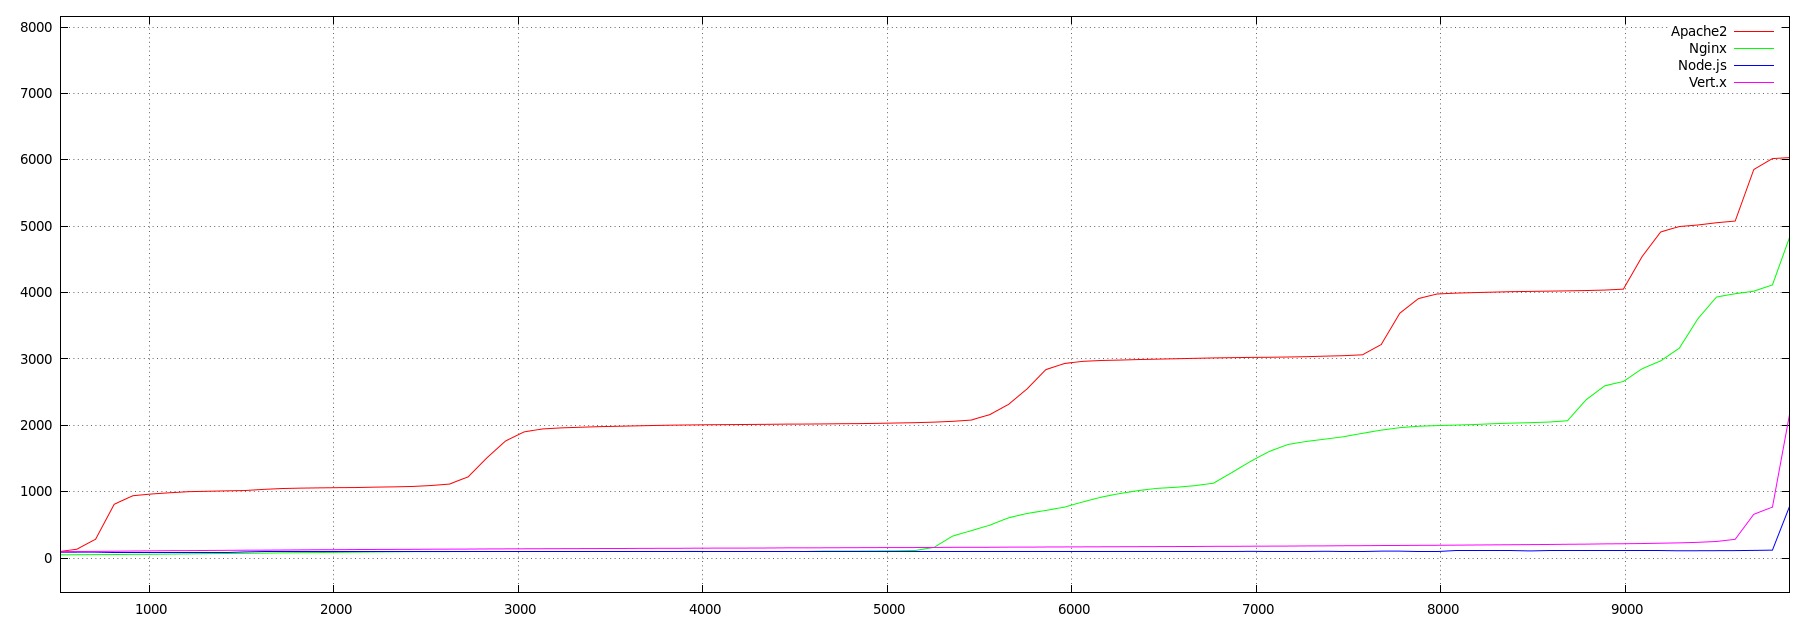
\includegraphics[width=\textwidth]{img/200kb_benchmark.png}
\caption[Plot of the web server benchmark results (all servers)]{Plot of the web server benchmark results between Apache2, Nginx, Node.js, Vert.x (x-axis: requests, y-axis: time in ms)}
\label{fig:benchmark_all}
\end{figure}

\begin{figure}[htbp]
\centering
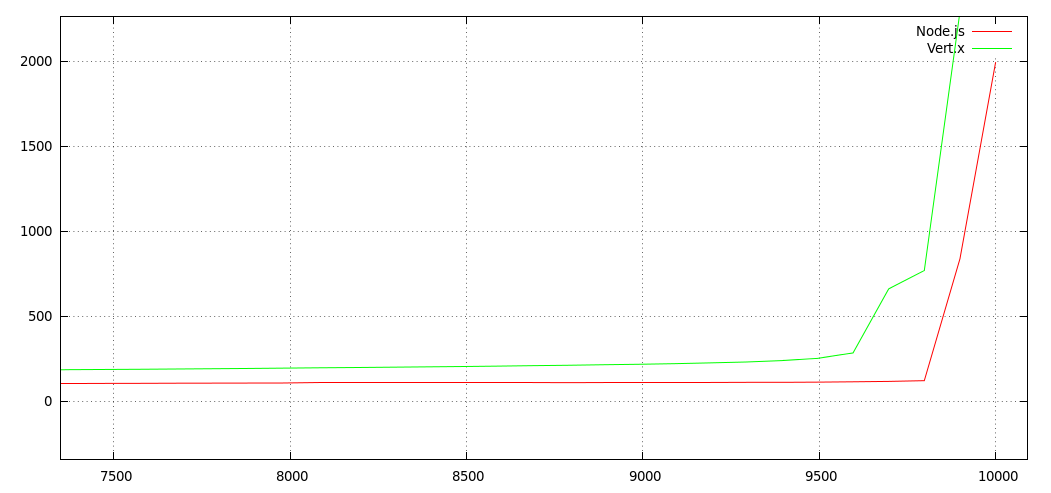
\includegraphics[width=\textwidth]{img/200kb_benchmark_node_vertx.png}
\caption[Plot of the web server benchmark results (asynchronous servers)]{Plot of the web server benchmark results between Node.js and Vert.x (x-axis: requests, y-axis: time in ms)}
\label{fig:benchmark_async}
\end{figure}


\paragraph{Scaling on a single machine}
Support for single machine scaling using multiple threads exists natively in
Vert.x and can be accomplished easily on a per-instance basis like shown in listing \ref{lst:starter_verticle}.
Each instance can
be deployed multiple times. This allows configurations like having one instance
for the main event loop and 4 instances for the worker verticles, so that
computation intense tasks can be handled by a thread pool of 4 threads. 
Vert.x provides  thread-safe data-structures that developers can use to share data between instances. However these data-structures are limited to immutable data types\footcite[Cf.][]{vertx_2012}\\

Node.js is designed to run single-threaded and can only scale to all available
cores by using the Cluster module\footcite[Cf.][]{node_2012b}, which is still in an experimental state.
This module allows to take advantage of a multi-core system by launching a cluster of Node.js processes to handle the load. Basically it enables the developer to run several worker processes (depending on the number of cores) and create an HTTP server for each of them, whereby all of them share one port. 


\paragraph{Scaling on distributed machines}
Vert.x uses Hazelcast's\footnote{See \url{http://www.hazelcast.com/}} clustering
functionality internally to scale on multiple machines.\\

\begin{lstlisting}[language=bash,caption={Starting a Vert.x application in cluster mode},label={lst:vertx_cluster}]
vertx run server.js -cluster -cluster-port 22000
\end{lstlisting}

Listing \ref{lst:vertx_cluster} shows how a Vert.x cluster can be set up on a
network with the default configuration. The cluster-port argument specifies on
which port distributed instances will communicate with each other and defaults
to $25500$ when omitted.
Each instance that is started in clustermode will have access to a distributed
event bus.\footcite[Cf.][]{vertx_2012} Implementation details on the cluster
internals can be found in the Hazelcast documentation on the project's
website.\\

Up to now, for Node.js there is no known way of distributing workloads among
different servers, however that wish was
addressed.\footcite[Cf.][]{node_clusterserver}


\paragraph{General ways of distributing workload among distributed machines}
One possible procedure is to deploy an application multiple times and to use an additional load balancer that
distributes incoming requests among all running deployments. This has some
implications: Due to the isolation in separate processes, application instances cannot share any
data or communicate directly with each other.
Furthermore, data might be stored in a physically separated database like CouchDb\footnote{See
\url{http://couchdb.apache.org/}} or in a key-value store like Redis\footnote{See
\url{http://redis.io/}}. This database could then potentially become a bottleneck when multiple application
processes require access, depending on its ability to address parallel processing.

\paragraph{Speeding up single requests}
Node.js and Vert.x do not offer any possibility to speed up a single request.
These requests will aways run at the same speed. What these frameworks do is to
maximise the number of possible requests while keeping the processing speed
steady. This is why it scales so well (see section \ref{scalability}). The only
additional delay between request and response is the time that a request waits
in the event loop until it gets processed.  In many cases however it is
desirable to minimize the computation time itself for a single request. Once
this is achieved it becomes a goal to keep that speed for a larger amount of
requests.\\


\section{Outlook}

This section is going to cover future prospects of the two technologies that were subject to investigation within this paper.\\

\paragraph{Node.js} Node.js, as became evident throughout the paper, is popular and enjoys healthy development. It is backed by a variety of modules that enable developers to implement complex functionality. The packaged modules available at \url{npmjs.org} indicate great interest, as the number of downloads (about 14.6 million last month\footcite[Cf.][]{node_packages}) suggests. In addition, the GitHub Commit History\footcite[Cf.][]{vertxcommithistory_2013} shows constant contributions. 

\paragraph{Vert.x} Recently there has been some uncertainty concerning the future
development of Vert.x, as recent news articles
indicate.\footcite[Cf.][]{Asay_2013} This is mainly related to the reaction of
VMware when Vert.x foudner Tim Fox left the company. Moreover, there is
currently no developer roadmap available that allows to infer the future
development. Its commit history on
GitHub\footcite[Cf.][]{vertxcommithistory_2013} is another sign of a decreasing
popularity, which, however has always been on a lower level than on GitHub but
might currently be related to the unclear future. It is likely that the development
activity for the Vert.x project starts increasing once it has completed the transition
 to the Eclipse foundation.

\paragraph{Evolving the Proof of Concept} The Proof of Concept introduced within this paper is an initial implementation that was set up to show the potential usage of asynchronous server technologies while remaining on a moderate level of complexity. However, the use case that was shown -- real-time insurance form infilling and instant price calculation based on inserted values -- provides great potential for companies to evolve their business model. The technology enables salesmen to interact more easily with clients and transforms geographically spread conclusion of contracts to the next stage, because the anonymity of web-based contracts can be mitigated by real-time communication that is not only limited to filling a form, but instead can be extended to live web-conferences with video/audio stream next to the form through the use of asynchronous server technologies. 

%
%
%
%
%
%OUTLOOK
%
%
%
%


\section{Conclusion}
\label{conclusion}

%----------------------------------------------------------------------------
% APPENDIX
%----------------------------------------------------------------------------
% Appendix sections need to be within the subappendices environment.
% Use the command \appsection{title} instead of \section to introduce each
% appendix. This will add each appendix to the list of appendices.

% sets the appendix environment and resets the section counters
\newpage \begin{appendices} 
\appendixtocon %adds an 'Appendices' entry to the toc

\appendixpage %prints the title on the page

\subsection*{\listappendixname}
%--------------------------------
% style of the \listofappendices command is defined in header.tex
\listofappendices

% begin appendices on a new page
\newpage

%start environment for subappendices, so that new sections are formatted as
%subsections of appendix
\begin{subappendices}
\renewcommand{\setthesubsection}{\arabic{subsection}:}%


\appsection{Middleware as use case for Node.js}
\label{middleware}
"The term middleware refers to the software layer between the operating system—including the basic communication protocols—and the distributed applications that interact via the network. This software infrastructure facilitates the
interaction among distributed software modules."\footcite[][]{Geihs_2001} This section is to point out briefly from a theoretical and practical perspective some of the aspects worth noting when dealing with Node.js and Vert.x as middleware.\\

The JVM\nomenclature{JVM}{Java Virtual Machine} and its associated libraries building the foundation for Vert.x are a classic example of this concept. The underlying concepts of both frameworks outlined thus far in this paper present advantages to middleware/library development as it does for business logic implementation. This realization manifests itself not only in the number of packages available on $npm$ (21,104 as of January 18, 2013)\footcite[Cf.][]{node_packages} but also in new projects built on top of Node.js.\\

One issue mentioned when dealing with middleware is the format of messages that are xexchanged among distributed systems.\footcite[149]{Tannenbaum_2007} As Node.js brings a typical client-side script language to the server-side, the developer can take advantage of that fact by using the universal format JavaScript Object Notation (JSON) and common exchange format by using "application/json" as content type.\footcite[Cf.][]{rfc4627} CouchDB, e.g., is a database storing documents in JSON and could benefit in particular from Node.js as middleware.\\

Furthermore, in section \ref{use_cases} the use case of Vert.x and Node.js as proxy server was outlined, which is another hint for the potential of those technologies in terms of middleware. Appendices \ref{appendix_kue}, \ref{app:etherpad} and \ref{appendix_meteor} will showcase what is possible when turning Node.js into a middleware-layer (fundamentally this is also true for Vert.x). 

\appsection{Kue – A Message Queue (Job Queue) based on Node.js}
\label{appendix_kue}

A message queue is “an area where you can add messages representing a task”\footcite[][2]{McGlennon_2007}. According to Microsoft Message Queue (MSMQ) it helps solve two basic problems:\footcite[Cf.][1]{McGlennon_2007}
\begin{itemize}
  \item Unavailability of communications with servers or clients, and 
  \item Communications between disparate systems and components.
\end{itemize}
Another use case for message queues is storing less-important information in a message queue while your DBMS is busy serving customers during the day.\footcite[Cf.][449]{Thomson_2002}
The basic concept behind message queues is as follows: When a message arrives from a client, the producer places it on a queue. It has then done its job and waits for the next input data. The consumer, which can be a process or application that may also be on a different server or even a different operating system\footcite[Cf.][2]{McGlennon_2007}, can then retrieve messages from the queue for processing (basically, the FIFO principle is applied).\footcite[Cf.][450]{Thomson_2002}
A common scenario for message queues is when only a little amount of requests create high loads on the server, e.g. video platforms such as Youtube or Vimeo.\footcite[Cf.][247]{Roden_2012} In such cases, it is useful to externalize CPU-intensive tasks in order not to impair responsiveness of the application.\footcite[Cf.][247]{Roden_2012}
Asynchronous server technologies such as Node.js can leverage message queues very well. As a feature of the event-driven model, an event handler is triggered when a new message is available. Thus, the queue does not need to be constantly polled for messages.\footcite[Cf.][]{Knight_2011}

Kue is an example of a message queue (also called job queue) that is entirely developed in Node.js. It uses redis as a queue server. With Kue, jobs can be prioritized, delayed, monitored graphically and in real-time, repeated if they failed and more. A key feature is the user interface to view and manage jobs in different states (queued, active, failed and completed). Kue can be installed easily according to Listing \ref{lst:installkue}.

\begin{lstlisting}[language=javascript,caption={Installing Kue via command-line},label=lst:installkue]
$ npm install kue $
\end{lstlisting}

\appsection{Case Study – LinkedIn}
\label{app:case_linkedin}
In 2012, LinkedIn, the career-oriented social network, has changed their back-end infrastructure of the mobile application, which was built on Ruby on Rails until then.\footcite[Cf.][]{Avram_2012} LinkedIn moved from Ruby on Rails to Node.js for performance and scalability reasons and has made immense performance improvements.\footcite[Cf.][]{ODell_2011} 
LinkedIn had scalability problems although less than 10% of their clients were using the mobile application.\footcite[Cf.][]{Avram_2012} Running on single-threaded Rails servers which caused that every request blocked the entire process, running Mongrel and leaking memory caused severe problems.\footcite[Cf.][]{Hoff_2012}
LinkedIn therefore wanted to implement an event-driven model and tested and evaluated three possible candidates: Rails/Event Machine, Python/Twisted, and Node.js.
Node.js was identified as the best solution for following benefits\footcite[Cf.][]{Avram_2012}:
\begin{itemize}
  \item Better performance (running up to 20x faster in certain scenarios) and lower memory overhead than other tested options, 
  \item Programmers could make use of their JavaScript skills. 
  \item Frontend JavaScript and backend mobile teams could be merged into a single unit. 
  \item Servers were cut from 30 to 3, leaving room to handle 10x current levels of resource utilization.
\end{itemize}

\appsection{Case Study – AIRCODE}
\label{app:case_aircode}

The following information are taken from the website of AIRCODE.\footnote{See aircode.co}
AIRCODE has implemented an application providing real-time news and visitor’s geolocation to the visitors of their website. The application is implemented in Node.js and aims to reveal the ability of Node.js of event-driven notification in real-time, i.e. in this specific case to deliver web pages with real-time news, based on live occurring events in six countries of the world. This is accomplished by providing the user with news from six countries at the same time – news being published in the moment the user receives them. The idea is to show that different news can be delivered at the same time, which makes use of Node.js’s strength of the underlying event-driven model.
Node.js fetches the news feeds and distributes them to every current visitor in real-time. When new visitors connect to the web site, all other visitors will be notified with the others’ position. For this, Node.js uses the broadcast function from the socket.io module.

\appsection{Case Study – Etherpad}
\label{app:etherpad}
On 22 August 2011 the Etherpad Lite, that is implemented with Node.js, was released.\footcite[Cf.][]{Martischka_2011}  Etherpad is an Open Source online editor providing collaborative editing of documents in real-time.\footnote{See etherpad.org} The original Etherpad had the following main problems:\footcite[Cf.][]{Martischka_2011} Resource utilization: – the JVM that Etherpad was based on, consumed 1-2 GB RAM during normal operation time. Besides memory leaks, infinite loops, constantly high server loads and server outages were other severe problems.
Peter Martischka, an Etherpad developer, migrated the entire application from Rhino to Node.js. It was a successful act. Node.js solved many problems in terms of performance and resource utilization. 

\appsection{Case Study – Clock, a UK web agency}
\label{app:case_clock}

The following information are taken from an online article\footnote{\url{http://venturebeat.com/2012/01/07/building-consumer-apps-with-node/}} on VentureBeat\footnote{\url{http://venturebeat.com/}} and are based on the statements by Paul Serby, CTO of Clock.
Clock is a web agency in the United Kingdom that builds the websites for their clients in Node.js. They chose Node.js for several reasons:
First, JavaScript as the underlying programming language of Node.js is very beneficial. Most developers at Clock have JavaScript expertise what makes it relatively easy to introduce Node.js and therefore saves time and costs. In addition to that, Clock uses MongoDB. Thus, code can be used on the browser-side, server-side and for the database as MongoDB uses JavaScript for querying data.\footnote{\url{http://www.mongodb.org/}}
Paul says that “our browser-side JavaScript code improved in quality and structure”. Another aspect the developers at Clock appreciate is the highly active community which is useful when solving programming issues. Also, the developers have had “large productivity gains in HTML and CSS using Jade and Stylus\footnote{\url{http://clock.co.uk/tech-blogs/a-simple-website-in-nodejs-with-express-jade-and-stylus}}”.
Furthermore, the amount of traffic could be increased with Node.js compared to PHP with Apache which was used before. Clock says that using Node.js and MongoDB they could scale up much better than with PHP and PostgreSQL. Moreover, Clock developers appreciate the many hosting options that come with Node.js (e.g. No.de, Joyent’s SmartMachine, Heroku and Nodejitsu). Joyent’s SmartMachine is supposed to be used for upcoming projects.\\
In conclusion, Clock states that at the beginning the projects took some extra time as developers had to get used to Node.js and the underlying concepts. However, Node.js fitted their use case very well (which was to develop high-scaling web applications) and after a short time, it made their development “extremely effective”.



\appsection{Meteor and Opa}
\label{appendix_meteor}
\FloatBarrier
Meteor and Opa are two frameworks built on top of Node.js and MongoDB created around a radically new development workflow. Both eliminate the distinction between client-side and server-side code, instead the developer writes code in a very similar way to conventional desktop programming.\footcite[Cf.][]{meteorDocs} The difference is that the framework provides functionality to that enables the code to alter its behavior depending on where it runs.\footcite[Cf.][]{meteorDocs} An example of this methodology can be found in appendix \ref{appendix_meteor}.

Meteor leverages Node.js enabling it to make use of its JavaScript-based concept and  the developer to take advantage of the variety of packages available for Node.js. Special attention should be paid to the fact that Meteor server code runs in one thread per request as opposed to the usual asynchronous callback methodology that applies to Node.js itself normally.\footcite[Cf.][]{meteorDocs} Through heavy integration of MongoDB (or Meteor's data layer in general) it is also unnecessary to write and handle AJAX calls manually as all data transmission (e.g.\ synchronization, publish, subscribe) is abstracted away.\footcite[Cf.][]{meteorDocs} The Meteor-provided example app 'leaderboard', whose code is provided in listings \ref{lst:leaderboard_html}\footcite[Cf.][]{leaderboard} and \ref{lst:leaderboard_js}\footcite[Cf.][]{leaderboard} (CSS\nomenclature{CSS}{Cascading Style Sheets} omitted), highlights this concept very well.

At its current stage it is an ideal prototyping environment for it allows ideas to be brought into usable form very quickly, even including hosting in the cloud. These capabilities are especially useful when creating single-page applications (i.e.\ JS UI\nomenclature{UI}{User Interface} with only one HTML page served). Currently this means that more complex software is much more difficult to build using Meteor especially if it requires serving multiple pages (e.g.\ public material, user area and administrative area). The POC\nomenclature{POC}{Proof Of Concept} implemented as part of this paper was originally planned to be built using Meteor, this however had to be shelved as undocumented errors arose. These quickly became unfixable as the error messages provided proved no help in debugging and conventional JS debuggers also were unable to provide assistance.
Trying to shoehorn Meteor into something it was not built for, this behavior is not unexpected.

Opa is conceptually similar although its technical underpinnings as well as the developer-used framework is different which is illustrated in fig. \ref{img:opa}.\footcite{opa}

\begin{figure}[hbtp]
\centering
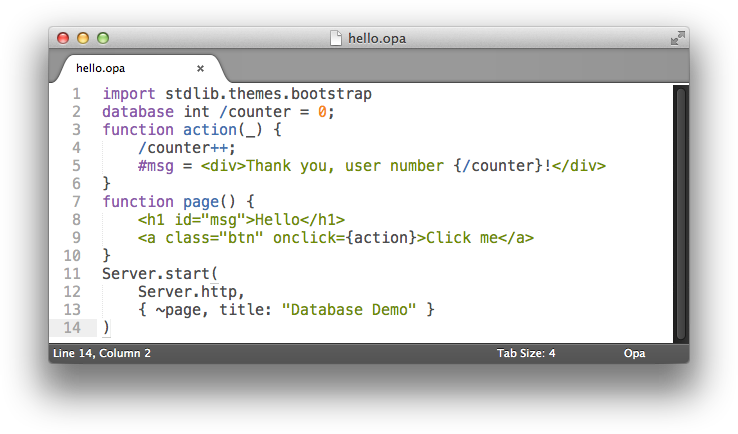
\includegraphics[scale=0.5]{img/hello-opa-write}
\caption{Opa example code \label{img:opa}}
\end{figure}

\lstinputlisting[float,
language=html,
morekeywords={template},
caption={HTML of the Meteor example 'Leaderboard'},
label=lst:leaderboard_html]{lst/leaderboard/leaderboard.html}

\lstinputlisting[float,
language=Javascript,
morekeywords={},
caption={JS of the Meteor example 'Leaderboard'},
label=lst:leaderboard_js]{lst/leaderboard/leaderboard.js}
\FloatBarrier 

\appsection{Benchmarking results}
\label{app:benchmark_results}
\lstinputlisting[numbers=none,caption={Benchmarking results as shown by the Apache benchmarking tool for web servers},
label={lst:benchmark_results}]{lst/200kb_benchmarks_output.txt}

%--------------------------------
% close the appendices environment
\end{subappendices}
\end{appendices}
